\begin{abstract}

  \textbf{1. }
    Phylogenetic trees are current routinely reconstructed from an alignment 
    of character sequences (usually nucleotide sequences). 
    Bayesian tools, such as MrBayes, RevBayes and BEAST2, 
    have gained much popularity over the last decade, 
    as they allow joint estimation of the posterior distribution of the 
    phylogenetic tree and the parameters of the underlying inference model.  
    An important ingredient of these Bayesian approaches is the species tree 
    prior. While in principle the Bayesian framework allows for comparing 
    different species tree priors and hence may elucidate the macroevolutionary 
    processes underlying the species tree, in practice only 
    macroevolutionary models that allow for fast computation of the prior 
    probability are used. 
    An open question is, how accurate the tree estimation is
    when the real macroevolutionary processes are substantially different 
    from those assumed in the tree prior. \\
  \textbf{2. }
    Here we present \verb;pirouette;, 
    a free, libre and open-source R package that assesses 
    the inference error made by Bayesian phylogenetics for a given 
    macroevolutionary diversification model. \verb;pirouette; makes use of 
    BEAST2, but its philosophy applies to any Bayesian phylogenetic inference 
    tool. \\
  \textbf{3. }
    We describe \verb;pirouette;'s usage and the biological scientific
    question it can answer, including full examples. \\
  \textbf{4. }
    Last, we discuss the results obtained by the examples and their interpretation. \\
\end{abstract}

{\bf Keywords:} computational biology, evolution, phylogenetics, tree prior, 
Bayesian model selection, BEAST2, babette, pirouette, R

%%%%%%%%%%%%%%%%%%%%%%%%%%%%%%%%%%%%%%%%%%%%%%%%%%%%%%%%%%%%%%%%%%%%%%%%%%%%%%%%
\section{Introduction}
%%%%%%%%%%%%%%%%%%%%%%%%%%%%%%%%%%%%%%%%%%%%%%%%%%%%%%%%%%%%%%%%%%%%%%%%%%%%%%%%

The development of new powerful Bayesian phylogenetic inference tools, 
such as BEAST [\cite{drummond2007beast}], 
MrBayes [\cite{huelsenbeck2001mrbayes}]
or RevBayes [\cite{hohna2016revbayes}], 
has been a major advance in constructing phylogenetic trees 
from character data (usually nucleotide sequences) extracted 
from extant (but also extinct) organisms, and hence in our understanding of the main drivers and modes of diversification.

BEAST [\cite{drummond2007beast}] is a typical Bayesian phylogenetics tool, 
that needs both character data and priors to infer a posterior distribution of phylogenies.
Specifically, for the species tree prior - which describes the process of diversification - 
BEAST has built-in priors such as the Yule [\cite{yule}] and 
(constant-rate) birth-death [\cite{nee1994reconstructed}] models.
These simple tree priors are most commonly used, as these 
have sufficient biological complexity, while being computationally fast.
BEAST's successor, BEAST2 [\cite{bouckaert2014beast}],
has a package manager, that allows third-party users to extend existing functionalities. For example, one can add novel diversification models by writing a BEAST2 package that contains the likelihood formula
of a phylogeny under the novel diversification model, i.e. the prior probability of a species tree.
Many such diversification models (and their associated probability algorithms) have been developed, e.g., models in which diversification is 
time-dependent [\cite{nee1994reconstructed}, \cite{rabosky2008explosive}], 
or diversity-dependent [\cite{etienne2011diversity}],
or where diversification rates change for specific lineages and their descendants [\cite{etienne2012conceptual}, 
\cite{rabosky2014automatic}, \cite{alfaro2009nine}, \cite{laudanno2018sls}], models that treat speciation as a process that takes 
time [\cite{rosindell2010protracted}][\cite{etienne2012prolonging}][\cite{lambert2015reconstructed}], 
or as a burst of simultaneous branching
events [\cite{laudanno2018mbd}], or where diversification rate
depends on a trait that has two [\cite{maddison2007estimating}], 
or more [\cite{fitzjohn2012diversitree}] states,
even concealed states [\cite{beaulieu2016detecting}] 
or a combination of all these [\cite{herrera2018detecting}].
Only a few of these diversification models are available as a BEAST2 package.

When a novel diversification model is introduced,
its performance in inference should be tested.
Part of a model's performance is its ability to recover parameters from simulated data with known parameters (e.g. [\cite{etienne2014estimating}]), where ideally the estimated parameter values closely match the known/true values.

Even when a diversification model passes the procedure described above,
it is not necessarily used in Bayesian inference.
Bayesian phylogenetic inference often requires that the prior probability of the phylogeny according to the diversification model has to be computed millions of times. Therefore, biologically interesting but computationally expensive tree priors are non-viable. This is not necessarily problematic, when the data are very informative, as this will reduce the influence of the tree prior.
However, the assumption that tree prior choice is of low importance must first be verified.

There have been multiple attempts to investigate the importance of tree
prior choice. For example, recently Sarver et al., [\cite{sarver2019choice}] 
showed that the choice of tree prior does not 
substantially affect phylogenetic inferences of diversification rates.
Also recently, Duchene et al. [\cite{duchene2018phylodynamic}] released
a BEAST2 package to assess how well posterior predictive simulations
recover a given tree when using the standard diversification models.
These studies show how current diversification models compare
to one another, but they do not help to assess the importance of a new tree prior. 

Here we introduce a method to quantify the importance of a novel tree prior.
The method starts with a phylogeny generated by the new model for the tree prior. Next, nucleotide sequences are simulated on this phylogeny. Then, using the tree priors built-in into BEAST2, a Bayesian posterior distribution of phylogenies is inferred. We can then compare the inferred and simulated phylogenies. How to properly perform this comparison forms the heart of our method.
Only new diversification models that result in a large discrepancy between inferred and simulated phylogenies will be worth the effort and computational burden 
to implement a species tree prior for in a Bayesian framework.

Our method is programmed as an R package called \verb;pirouette;.
\verb;pirouette; is built on \verb;babette; [\cite{bilderbeek2018babette}], 
which calls BEAST2 [\cite{bouckaert2014beast}]. 

%%%%%%%%%%%%%%%%%%%%%%%%%%%%%%%%%%%%%%%%%%%%%%%%%%%%%%%%%%%%%%%%%%%%%%%%%%%%%%%%
\section{Description}
%%%%%%%%%%%%%%%%%%%%%%%%%%%%%%%%%%%%%%%%%%%%%%%%%%%%%%%%%%%%%%%%%%%%%%%%%%%%%%%%

\verb;pirouette; is written in the R programming language (\cite{R}).
The goal of \verb;pirouette; is to quantify the importance of a tree prior.
It does so by measuring the inference error made for a given reconstructed phylogeny, 
simulated under a (usually novel) diversification model.
We refer to the true prior that generated the given tree
as the 'generative tree prior' $\mathit{p_{G}}$.
Many tree priors have a parameter setting for which it reduces to a standard tree prior. For example, a protracted birth-death model reduces to a standard birth-death model when speciation-completion rate approaches infinity [i.e. rate $\lambda$ in \cite{etienne2014estimating}, eqs.~(2b) and (2c)].
When benchmarking a novel tree prior, 
one will typically construct phylogenies 
for different combinations of the diversification model's parameters, 
to assess under which scenarios the inference error cannot be neglected. 
While we recommend many replicate simulations when assessing a novel tree prior, our examples contain only one replicate as they are for illustrative purposes only.

\verb;pirouette; is very flexible and allows the user 
to specify a wide variety of custom settings. 
These settings can be grouped in macro-sections, 
according to how they operate in the pipeline. 
We summarize them in Table~\ref{tab:options} and Table~\ref{tab:definitions}.

Although many possible tests can be performed, 
we show the usage of \verb;pirouette; by a story that introduces
its features gradually, yet ending in quantifying the impact a tree prior has
in Bayesian inference.

\begin{sidewaystable}
\centering
  \begin{tabular}{|p{3.4cm}|p{9.7cm}|p{4.5cm}@{}|}
    \hline
    \centering
    %%%%%%%%%%%%%%%%%%%%%%%%%%%%%%%%%%%%%%%%%%%%%%%%%%%%%%%%%%%%%%%%%%%%%%%%%%%%
    \textbf{Sub-argument} & 
    \textbf{Description} &
    \textbf{Possible values} \\ 
    \hline
    %%%%%%%%%%%%%%%%%%%%%%%%%%%%%%%%%%%%%%%%%%%%%%%%%%%%%%%%%%%%%%%%%%%%%%%%%%%%
    \verb;tree_prior; &
    Macroevolutionary diversification model &
    Yule, BD, CBS, CCP, CEP \\
    %%%%%%%%%%%%%%%%%%%%%%%%%%%%%%%%%%%%%%%%%%%%%%%%%%%%%%%%%%%%%%%%%%%%%%%%%%%%
    \verb;clock_model; &
    Clock for the DNA mutation rates &
    strict, relaxed log-normal \\
    %%%%%%%%%%%%%%%%%%%%%%%%%%%%%%%%%%%%%%%%%%%%%%%%%%%%%%%%%%%%%%%%%%%%%%%%%%%%
    \verb;site_model; &
    Nucleotide substitution model &
    JC, HKY, TN93, GTR \\
    %%%%%%%%%%%%%%%%%%%%%%%%%%%%%%%%%%%%%%%%%%%%%%%%%%%%%%%%%%%%%%%%%%%%%%%%%%%%
    \verb;mutation_rate; &
    Pace at which mutation occurs &
    \verb;mutation_rate; $\in \mathbb{R}_{>0}$\\
    %%%%%%%%%%%%%%%%%%%%%%%%%%%%%%%%%%%%%%%%%%%%%%%%%%%%%%%%%%%%%%%%%%%%%%%%%%%%
    \verb;root_sequence; &
    DNA sequence at the root of the tree &
    any combination of a, c, g, t \\
    %%%%%%%%%%%%%%%%%%%%%%%%%%%%%%%%%%%%%%%%%%%%%%%%%%%%%%%%%%%%%%%%%%%%%%%%%%%%
    \verb;model_type; &
    Criterion to select an inference model &
    Generative, Candidate \\
    %%%%%%%%%%%%%%%%%%%%%%%%%%%%%%%%%%%%%%%%%%%%%%%%%%%%%%%%%%%%%%%%%%%%%%%%%%%%
    \verb;run_if; &
    Condition under which an inference model is used &
    Always, Best candidate \\
    %%%%%%%%%%%%%%%%%%%%%%%%%%%%%%%%%%%%%%%%%%%%%%%%%%%%%%%%%%%%%%%%%%%%%%%%%%%%
    \verb;do_measure_evidence; &
    Sets whether or not the evidence of the model is to be computed &
    TRUE, FALSE \\
    %%%%%%%%%%%%%%%%%%%%%%%%%%%%%%%%%%%%%%%%%%%%%%%%%%%%%%%%%%%%%%%%%%%%%%%%%%%%
    \verb;error_function; &
    Specifies how to measure the error &
    nLTT, $|\gamma|$ \\
    %%%%%%%%%%%%%%%%%%%%%%%%%%%%%%%%%%%%%%%%%%%%%%%%%%%%%%%%%%%%%%%%%%%%%%%%%%%%
    \verb;burn_in_fraction; &
    Specifies the percentage of initial posterior trees to discard &
    \verb;burn_in_fraction; $\in [0, 1]$\\
    %%%%%%%%%%%%%%%%%%%%%%%%%%%%%%%%%%%%%%%%%%%%%%%%%%%%%%%%%%%%%%%%%%%%%%%%%%%%
    \hline
  \end{tabular}
  \caption{
    Most important parameter options.
    Yule = pure birth model (\cite{yule})
    BD = birth death (\cite{nee1994reconstructed}), 
    CBS = coalescent Bayesian skyline (\cite{drummond2005bayesian}), 
    CCP = coalescent constant-population, 
    CEP = coalescent exponential-population,
    JC = Jukes and Cantor (\cite{jukes1969evolution}), 
    HKY = Hasegawa, Kishino and Yano (\cite{hasegawa1985dating}), 
    TN93 = Tamura and Nei (\cite{tamura1993estimation}), 
    GTR = Generalized time-reversible model (\cite{tavare1986some}).
  }
  \label{tab:options}
\bigskip

  \begin{tabular}{|@{}c|p{4cm}|p{12.2cm}|}
    \hline
    \centering
    %%%%%%%%%%%%%%%%%%%%%%%%%%%%%%%%%%%%%%%%%%%%%%%%%%%%%%%%%%%%%%%%%%%%%%%%%%%%
    \textbf{Symbol} &
    \textbf{Macro-argument} &
    \textbf{Description} \\
    \hline
    %%%%%%%%%%%%%%%%%%%%%%%%%%%%%%%%%%%%%%%%%%%%%%%%%%%%%%%%%%%%%%%%%%%%%%%%%%%%
    $\mathit{G}$ &
    Generative model &
    The full setting to produce BEAST2 input data. 
    Its core features are the tree prior $\mathit{p_{G}}$, the clock 
    model $\mathit{c_{G}}$ and the site model $\mathit{s_{G}}$. \\
    %%%%%%%%%%%%%%%%%%%%%%%%%%%%%%%%%%%%%%%%%%%%%%%%%%%%%%%%%%%%%%%%%%%%%%%%%%%%  
    $\mathit{A}$ &
    Alignment model &
    It includes the parts of the generative model that directly affect the 
    alignment generation, like the clock model $\mathit{c_{G}}$ and 
    the site model $\mathit{s_{G}}$. Additional arguments can be provided, 
    such as the mutation rate and the root sequence. \\
    %%%%%%%%%%%%%%%%%%%%%%%%%%%%%%%%%%%%%%%%%%%%%%%%%%%%%%%%%%%%%%%%%%%%%%%%%%%%
    $\mathit{X_{i}}$ &
    $i$-th candidate experiment &
    Full setting for a Bayesian inference. It is made by a 
    candidate inference model $\mathit{I_{i}}$ and its 
    inference conditions $\mathit{C_{i}}$. \\
    %%%%%%%%%%%%%%%%%%%%%%%%%%%%%%%%%%%%%%%%%%%%%%%%%%%%%%%%%%%%%%%%%%%%%%%%%%%%
    $\mathit{I}$ &
    Inference model &
    Phylogenetic inference model to run BEAST2. Likewise the generative model $G$, 
    its main components are the tree prior $\mathit{p_{I}}$, the clock model $\mathit{c_{I}}$ and the site model $\mathit{s_{I}}$. \\
    %%%%%%%%%%%%%%%%%%%%%%%%%%%%%%%%%%%%%%%%%%%%%%%%%%%%%%%%%%%%%%%%%%%%%%%%%%%%
    $\mathit{C}$ & Inference conditions & Conditions under which $\mathit{I}$ 
    is used in the inference. 
    They are composed by the model type, run condition and 
    whether to measure the evidence. \\
    %%%%%%%%%%%%%%%%%%%%%%%%%%%%%%%%%%%%%%%%%%%%%%%%%%%%%%%%%%%%%%%%%%%%%%%%%%%%
    $\mathit{E}$ & Error measure parameters & 
    Errors measurement setup that can be specified providing an 
    error function to measure the difference between the original phylogeny 
    and the inferred posterior. The initial part of the posterior that is 
    reckoned as not representative can be discarded using a burn-in fraction. \\
    %%%%%%%%%%%%%%%%%%%%%%%%%%%%%%%%%%%%%%%%%%%%%%%%%%%%%%%%%%%%%%%%%%%%%%%%%%%%
    \iffalse
    $\mathit{T}$ & Twinning parameters & Twin tree creation procedure & 
      $\mathit{\tau_{p}}$ \\
    %%%%%%%%%%%%%%%%%%%%%%%%%%%%%%%%%%%%%%%%%%%%%%%%%%%%%%%%%%%%%%%%%%%%%%%%%%%%
    \fi
    \hline 
  \end{tabular}
  \caption{
    Definitions of terms and relative symbols used in the main text and in 
    Fig~\ref{fig:pipeline}. To run the pipeline $\mathit{A}$, $\mathit{X}$ 
    and $\mathit{E}$ must be specified. Examples can be found in 
    listings~\ref{lst:create_alignment_params}, 
    \ref{lst:create_gen_experiment_explicit} and 
    \ref{lst:create_error_measure_params}.
  }
  \label{tab:definitions}
\end{sidewaystable}

\subsection{pirouette's pipeline}
\label{subsec:pipeline}

\begin{figure}
  \centering
  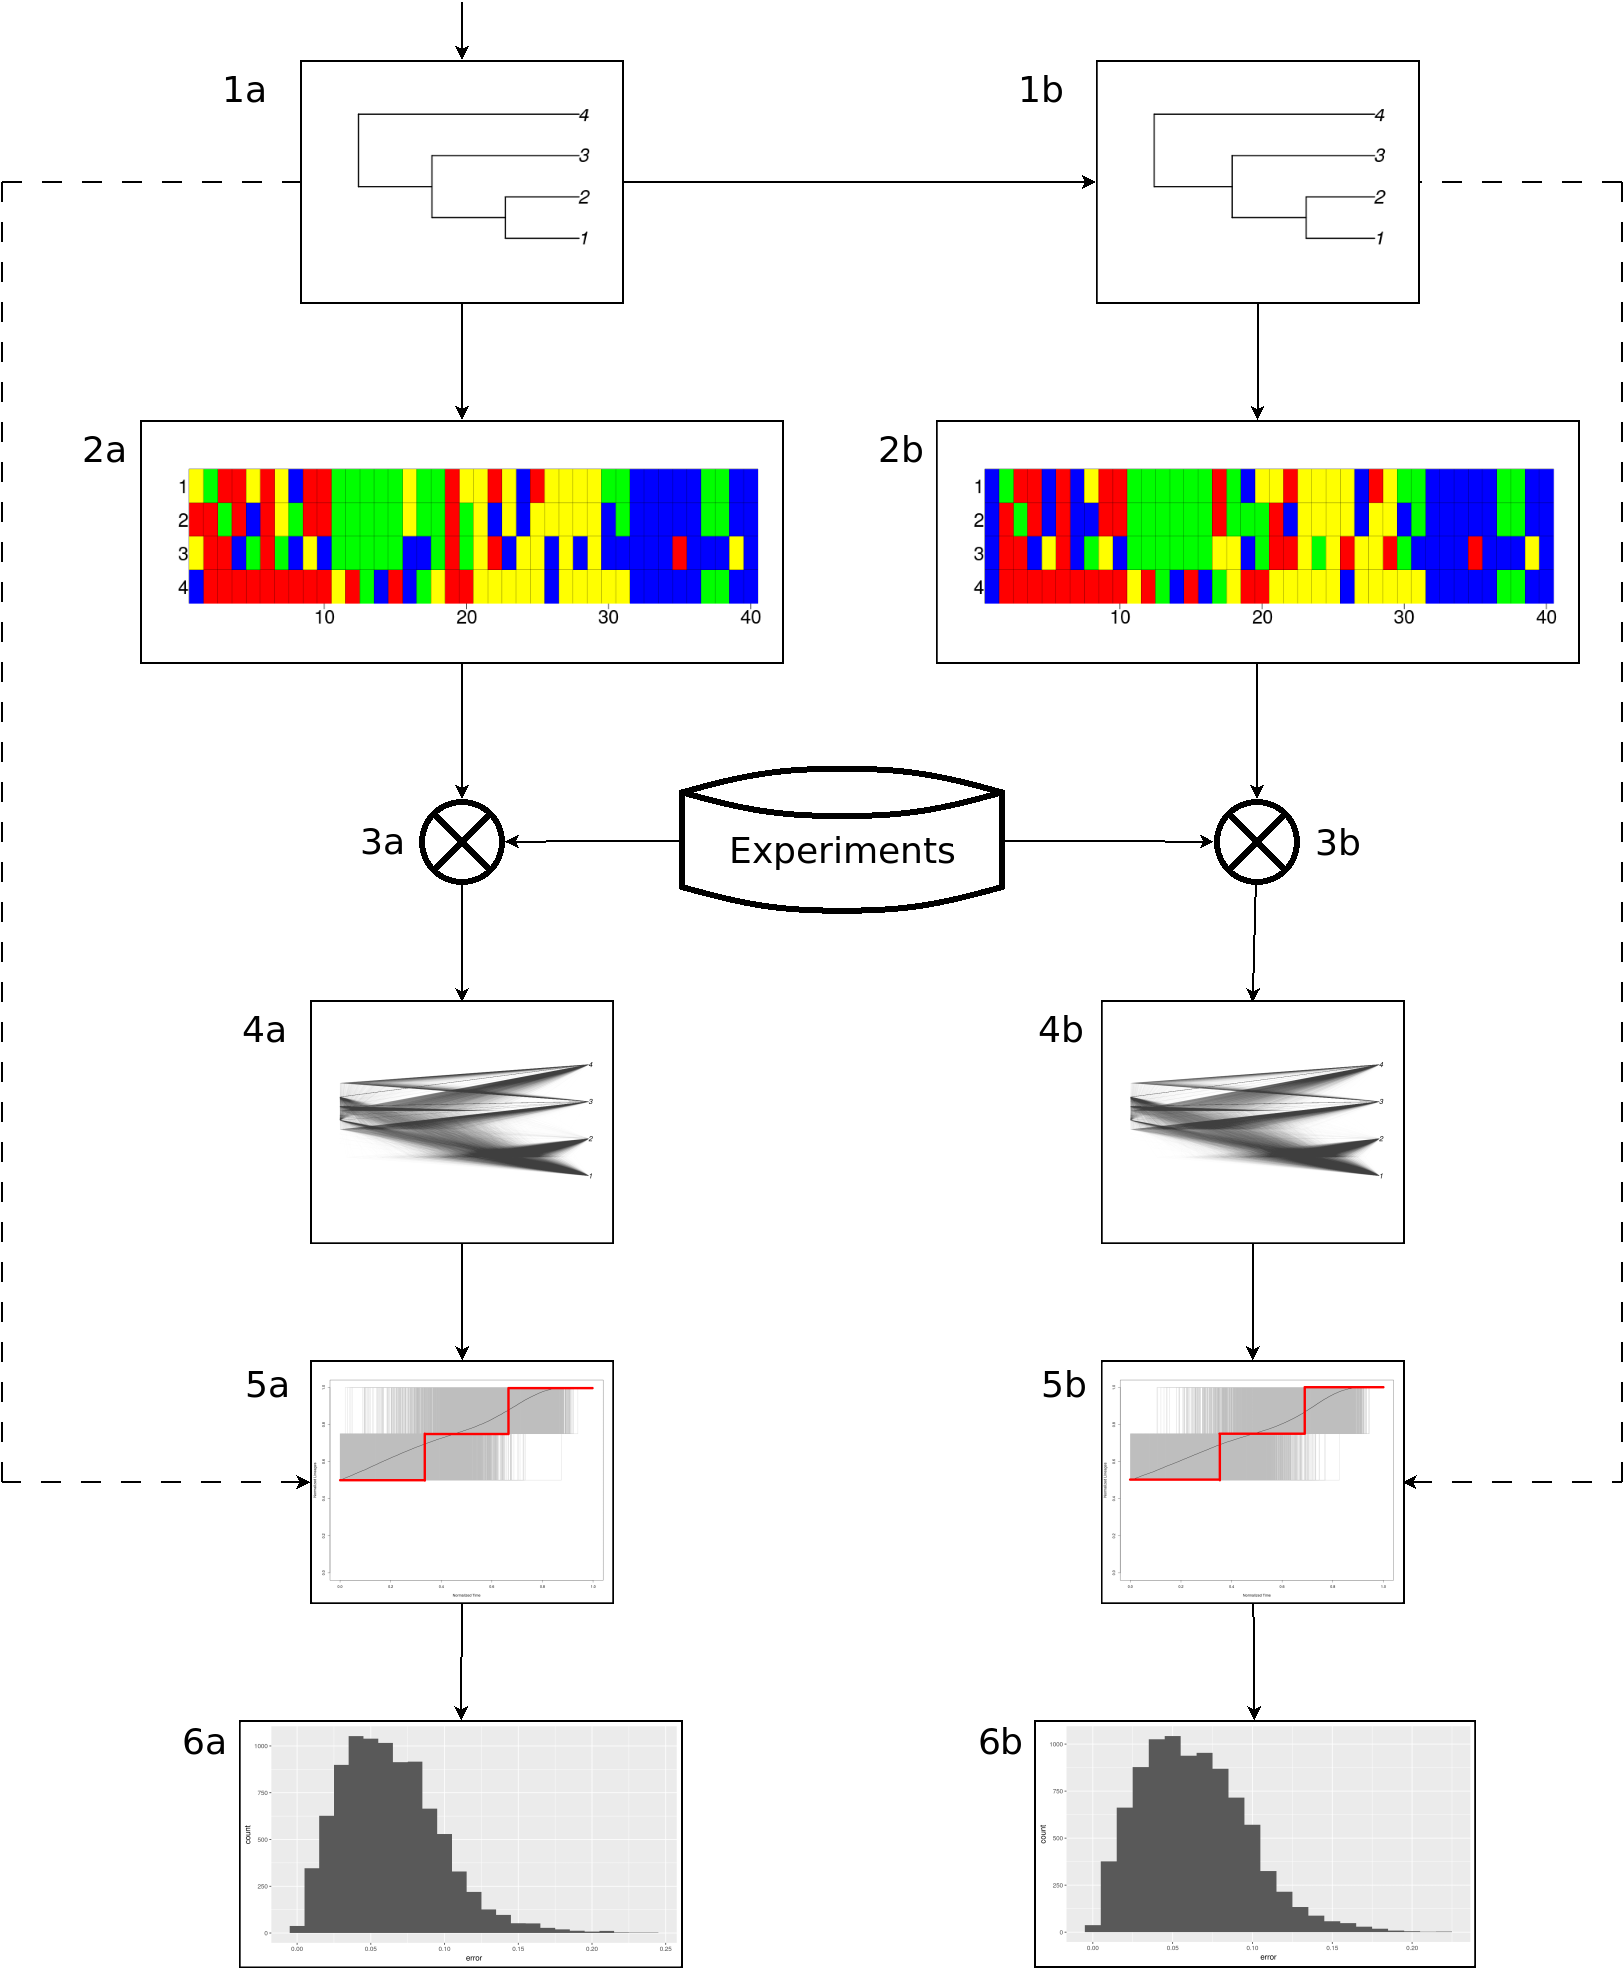
\includegraphics[width = \textwidth]{workflow.png}
  \caption{
    \texttt{pirouette} pipeline.
    The pipeline starts from a phylogeny (1a) simulated by the generative tree prior 
    $\mathit{p_{G}}$.
    The phylogeny is converted to an alignment (2a) using the generative alignment model 
    $\mathit{A} = (\mathit{c_{G}}, \mathit{s_{G}})$, composed by a clock and a site model. 
    The user supplies one or more experiments.
    For each candidate experiment $\mathit{X_{i}}$ 
    (a tuple of inference model $\mathit{I_{i}}$ and condition $\mathit{C_{i}}$),
    if its condition $\mathit{C_{i}}$ is 
    satisfied (which can depend on the alignment), 
    the corresponding inference model $\mathit{I} = \mathit{I_{i}}$ is selected 
    to be used in the next step.
    The inference models (3) of the selected experiments use the alignment (2a) 
    to each create a Bayesian posterior of (parameter estimates and) 
    phylogenies (4a). 
    Each of the posteriors' trees is compared to the true phylogeny (1a) 
    using error measure $\mathit{E}$, 
    resulting in an error distribution (5a). 
    Optionally, for each selected inference model a twin pipeline can be run.
    A twin phylogeny (1b) can be generated from the original 
    phylogeny (1a) using the tree prior $\mathit{p_{I}}$ of the selected inference model (3).
    Analogously, a twin alignment is simulated from the twin phylogeny along with clock model $\mathit{c_{I}}$ and site model $\mathit{s_{I}}$ imported from the selected inference model.
    The twin pipeline mimics the procedure of the main pipeline, resulting in a twin error distribution (5b).
  }
  \label{fig:pipeline}
\end{figure}

We assume the user has a phylogeny simulated with the new diversification model. The pipeline to assess the error BEAST2 makes in inferring this phylogeny then contains the following steps:
\begin{enumerate}
  \item from the given phylogeny an alignment is simulated 
    under a known alignment model $\mathit{A}$;
  \item from this alignment, according to the specified inference conditions $\mathit{C}$, 
    an inference model $\mathit{I}$ is picked (which may differ from the 
    generative model);
  \item the inference model and the alignment are used 
    to infer a posterior distribution of phylogenies;
  \item the phylogenies in the posterior are compared with the given phylogeny 
    to estimate the error made, according to the error measure $\mathit{E}$ specified 
    by the user;
\end{enumerate}
The pipeline is visualized in Fig.~\ref{fig:pipeline}. 
There is also the option to generate a 'twin tree', 
that goes through the same pipeline. 
The utility of this twin tree will be explained below.

The first step simulates a DNA alignment from a given 
phylogeny (Fig.~\ref{fig:pipeline}, 1a $\rightarrow$ 2a)
using the DNA alignment parameters.
The DNA alignment parameters consist of a (DNA) root sequence, a (DNA) mutation rate, a clock model and a nucleotide substitution
model, which will be referred to as site model.
The root sequence is the DNA sequence of the shared common ancestor,
and is set to four equally-sized mononucleotide blocks by default, as this
helps interpreting the resulting alignment.
Supported site models are JC, HKY, TN and GTR. Only the strict
clock model is currently supported in this step.

The second step (Fig.~\ref{fig:pipeline}, 3)
selects one or more inference models $I$ from a set of inference 
models $I_{1},\dots,I_{n}$. 
We define an experiment $X_{i}$ as the combination of 
an inference model $I_{i}$ and the conditions $C_{i}$ 
to actually use it in the inference step.
For example, we may require that an inference
model (a combination of a tree prior, clock model and site model) 
should include the generative/true tree prior. 
As a second example, we may require that we have selected a set of 
candidate inference models,
of which only the best should be used in the actual inference.
In the first example, we specified the condition $C_{i}$ that this
generative model should always be run, whereas in the second example,
we specified condition $C_{i}$ that a candidate model should only be run
when being the best.
A 'best' model is defined as the inference model with
the highest evidence (a.k.a. marginal likelihood), given the alignment 
simulated in the previous step.
The evidence of an inference model is estimated by nested 
sampling [\cite{maturana2018model}], using the \verb;NS; BEAST2 package. We note that scripted use of BEAST2 packages is only possible under Linux and Mac.
Windows systems can do the model comparison for shorter DNA sequences 
using the web interface of \verb;mcbette; [\cite{mcbette}].

The third step infers the posteriors,
using the simulated alignment (Fig.~\ref{fig:pipeline}, 2a $\rightarrow$ 4a),
and the inference models that were selected in the previous step (3). 
For each selected experiment a posterior is inferred, using the 
\verb;babette; [\cite{bilderbeek2018babette}] R package which makes use of BEAST2. 
This step usually takes up most of the full pipeline's computation time.

The fourth step quantifies the inference error made. First the burn-in fraction is removed, i.e. the first phase of the Markov chain Monte Carlo (MCMC) run,
in which it samples an unrepresentative part of state space. By default, \verb;pirouette; 
removes the first 10\% of the posterior.
From the remaining posterior \verb;pirouette; 
creates an error distribution, by measuring the difference
between the true tree and each of the posterior 
trees (Fig.~\ref{fig:pipeline}, 4a $\rightarrow$ 5a).
The default way to quantify the difference between two phylogenies
is the nLTT statistic (\cite{janzen2015approximate}), but any 
user-defined error statistic can be used.

\subsection{Twin tree}\label{subsec:twinning}

An optional step is to generate a 'twin tree' $\tau_{I}$
(Fig.~\ref{fig:pipeline}, 1a $\rightarrow$ 1b)
and 'twin alignment'
that will be analyzed in the same way as the true tree (and alignment).
We define a phylogeny $\tau$ as the combination of
branching times $\Vec{t}$ and topology $\psi$.
Assuming that a non-standard generative prior $\mathit{p_{G}}$
produces a tree $\tau_{\mathit{G}}$,
with branching times $\Vec{t}_{\mathit{G}}$ and 
topology $\psi_{\mathit{G}}$, the twinning process T, in accordance with a chosen inference 
model $\mathit{I}$, creates a tree $\tau_{\mathit{I}}$
with branching times $\Vec{t}_{\mathit{I}}$ while preserving the 
topology $\psi_{\mathit{G}}$:
\begin{align}
  \tau_{\mathit{G}} = (\Vec{t}_{\mathit{G}}, \psi_{\mathit{G}}) 
  \xrightarrow[]{\mathit{T}} 
  \tau_{\mathit{I}} = (\Vec{t}_{\mathit{I}}, \psi_{\mathit{G}})
\end{align}
To achieve this, we find the parameters $\theta^{*}_{\mathit{I}}$ 
(e.g. speciation and extinction rates, in case of a birth-death model) 
that maximize the likelihood $L_{\mathit{I}}$ applied 
to the true tree, conditioned on its number of tips $n_{\mathit{G}}$,
where $L_{\mathit{I}}$ is the likelihood function  
associated with the chosen inference model $\mathit{I}$:
\begin{align}
    \max[L_{\mathit{I}}(\theta_{\mathit{I}}|\tau_{\mathit{G}}, n_{\mathit{G}})] 
\rightarrow \theta^{*}_{\mathit{I}}.
\end{align}
We use $\theta^{*}_{\mathit{I}}$ to simulate an equal number 
$n_{\mathit{I}} = n_{\mathit{G}}$ 
of branching times $\Vec{t}_{\mathit{I}}$ for the twin tree 
$\tau_{\mathit{I}}$, under the process $\mathit{I}$, 
while preserving the same topology.

From the twin tree, we simulate an alignment following the same
history as the twin tree, with the addition that 
the same total number of mutations have
taken place from root sequence to the sequences in the present.
This addition assures there is the same amount of historical information
stored in both the true and twin alignments.
We achieve this by simply simulating twin alignments until we
obtain one that has the desired number of mutations.

The twin tree serves as a control: even when the generating and inference models are identical, the posterior distribution of inferred trees will differ from the true tree due to stochasticity in producing an alignment and in MCMC sampling of the posterior; the twin tree provides this minimum error. We therefore need to compare the error distributions of $\tau_{\mathit{G}}$ and 
$\tau_{\mathit{I}}$. 
By imposing the same topology and the same number of mutations in the alignments, the differences in error distributions of the true tree and the twin tree are the consequence of different phylogenies (produced by different processes) and tree priors for the two parallel 
pipelines: the main pipeline uses the tree $\tau_{\mathit{G}}$ and a
possibly mismatched prior $\mathit{G}$, whereas the twin pipeline
uses the tree $\tau_{\mathit{I}}$ for a matching prior $\mathit{I}$.
So, for the twin trees, if the process is repeated a sufficient number of times, the resulting error distribution cannot be 
attributed to a mismatch between the true tree prior and the tree prior used in
inference.

%%%%%%%%%%%%%%%%%%%%%%%%%%%%%%%%%%%%%%%%%%%%%%%%%%%%%%%%%%%%%%%%%%%%%%%%%%%%%%%%
\section{Installation}
%%%%%%%%%%%%%%%%%%%%%%%%%%%%%%%%%%%%%%%%%%%%%%%%%%%%%%%%%%%%%%%%%%%%%%%%%%%%%%%%

\verb;pirouette; will be made available on CRAN from which it can then be easily installed:
\begin{lstlisting}[language=R, floatplacement=ht, frame=single]
install.packages("pirouette")
\end{lstlisting}

Until it is on CRAN, and for the most up-to-date version, 
one can download and install the package from \verb;pirouette;'s GitHub 
repository:

\begin{lstlisting}[
    language = R,
    floatplacement = ht,
    frame = single
]
usethis::install_github("richelbilderbeek/pirouette")
\end{lstlisting}
To start using \verb;pirouette;, load its functions in the global namespace first:
\begin{lstlisting}[language=R, floatplacement=ht, frame=single]
library(pirouette)
\end{lstlisting}
Because \verb;pirouette; calls BEAST2, BEAST2 must be installed. 
This can be done from within R, using:
\begin{lstlisting}[language=R, floatplacement=ht, frame=single]
install_beast2()
\end{lstlisting}
For the option to select the best candidate model,
\verb;pirouette; needs the "NS" BEAST2 package [\cite{maturana2018model}].
It can be installed from within R, using:
\begin{lstlisting}[language=R, floatplacement=ht, frame=single]
install_beast2_pkg("NS")
\end{lstlisting}

An overview of \verb;pirouette;'s main functions is shown in 
Table~\ref{tab:functions}. 
Their usage is demonstrated in the example code below.
All \verb;pirouette;'s functions are documented,
have a useful example and sensible defaults.

%%%%%%%%%%%%%%%%%%%%%%%%%%%%%%%%%%%%%%%%%%%%%%%%%%%%%%%%%%%%%%%%%%%%%%%%%%%%%%%%
\begin{table}[h]
  \centering
  \begin{tabular}{ | l | l | l | }
    \hline
    \textbf{Name} & \textbf{Description} & \textbf{Listing} \\
    \hline
    \verb;pir_run; & Run \verb;pirouette; & \ref{lst:pir_run} \\
    \verb;pir_plot; & Show the \verb;pirouette; results as a plot & \ref{lst:pir_plot} \\
    \verb;create_pir_params; & Create the \verb;pirouette; parameters & \ref{lst:create_pir_params} \\
    \hline
    \verb;create_alignment_params; & Create the alignment parameters & \ref{lst:create_alignment_params} \\
    \verb;create_twinning_params; & Create the twinning parameters & \ref{lst:create_twinning_params} \\
    \verb;create_experiment; & Create one experiment & \ref{lst:create_gen_experiment_explicit} \\
    \verb;create_error_measure_params; & Create the error measurement parameters & \ref{lst:create_error_measure_params} \\
    \hline
  \end{tabular}
  \caption{
    \texttt{pirouette}'s main functions, description and the number of the 
    listing in which it is used. 
  }
  \label{tab:functions}
\end{table}
%%%%%%%%%%%%%%%%%%%%%%%%%%%%%%%%%%%%%%%%%%%%%%%%%%%%%%%%%%%%%%%%%%%%%%%%%%%%%%%%

%%%%%%%%%%%%%%%%%%%%%%%%%%%%%%%%%%%%%%%%%%%%%%%%%%%%%%%%%%%%%%%%%%%%%%%%%%%%%%%%
\section{Usage}
%%%%%%%%%%%%%%%%%%%%%%%%%%%%%%%%%%%%%%%%%%%%%%%%%%%%%%%%%%%%%%%%%%%%%%%%%%%%%%%%

We show the usage of \verb;pirouette; by gradually introducing
its features.
First, to get an idea of the baseline error, 
we measure the Bayesian inference error when we start from a phylogeny 
generated under a known and standard tree prior.
Second, to establish that the true tree prior is indeed the best, 
we also measure the inference error made adopting a
best candidate inference model.
Lastly, we quantify the impact of the tree prior in the Bayesian inference. 
We do so by separating the baseline error from the complete error 
running the pipeline starting from a tree generated by an unknown 
or non-standard tree prior.

%%%%%%%%%%%%%%%%%%%%%%%%%%%%%%%%%%%%%%%%%%%%%%%%%%%%%%%%%%%%%%%%%%%%%%%%%%%%%%%%
\subsection{Generative model only}
%%%%%%%%%%%%%%%%%%%%%%%%%%%%%%%%%%%%%%%%%%%%%%%%%%%%%%%%%%%%%%%%%%%%%%%%%%%%%%%%

\verb;pirouette; quantifies the influence of a new tree prior on BEAST2's 
inference by measuring the discrepancy between a given tree and a posterior 
distribution of phylogenies obtained as result of the inference process. 
Due to stochasticity, posterior trees will generally differ from the given 
phylogeny $\tau_{\mathit{G}}$, even when the generative tree 
prior $\mathit{p_{G}}$ and alignment model $\mathit{A}$ are the same as those 
in the inference model $\mathit{I}$.
Measuring this difference allows us to know the baseline error
of the \verb;pirouette; pipeline. We therefore define as 'standard tree priors' 
all the tree priors that are available to be used within an inference model (see Table~\ref{tab:options}).

Now we can formulate the first example research question that \verb;pirouette; 
can answer: "What is the inference error made on phylogenies created by a 
standard diversification model?"

In this example we use a standard generative tree prior $\mathit{p_{G}^0}$, namely the Yule (pure-birth) tree prior. 
We choose to use a small tree with six taxa, to keep
the calculations short and the figure more readable.
We pick a crown age of ten time units. This value is 
completely arbitrary, but it ties in with the mutation rate 
used in simulating an alignment in the next step.

\begin{lstlisting}[
    language = R,
    floatplacement = ht,
    frame = single, 
    label = {lst:create_yule_tree}, 
    caption = {
      Create a Yule tree. 
      The resulting tree is shown in Figure~\ref{fig:yule_tree}.
    }
  ]
phylogeny <- create_yule_tree(n_taxa = 6, crown_age = 10)
\end{lstlisting}

\begin{figure}[ht]
  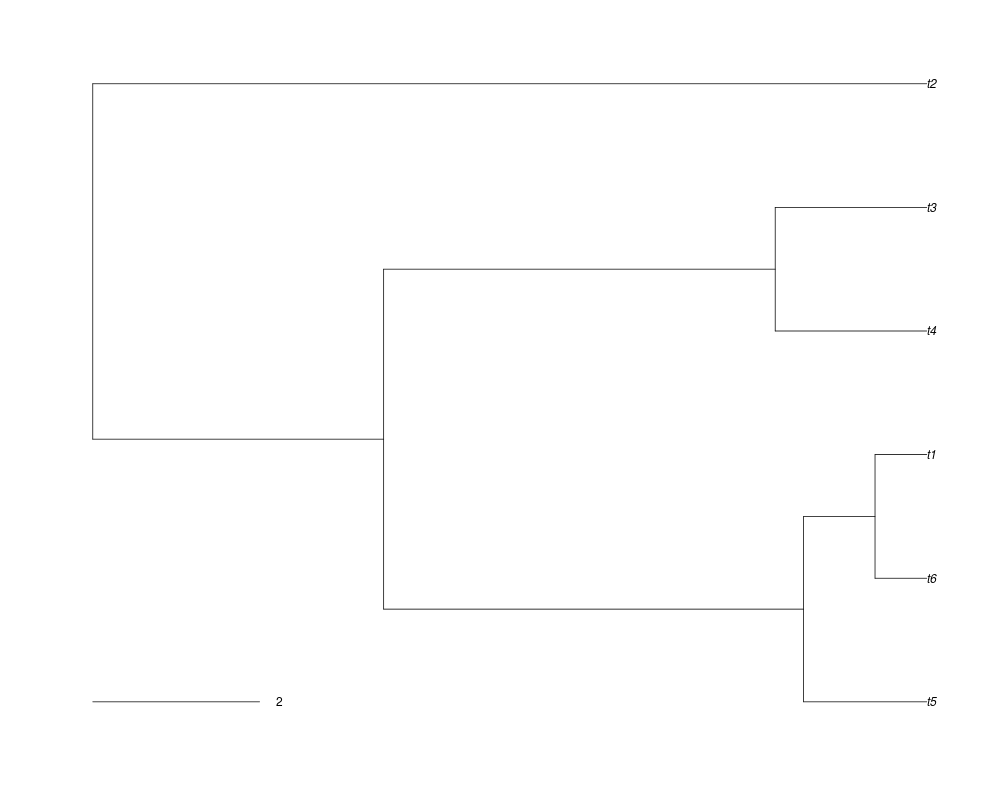
\includegraphics[width=\textwidth]{example_1/true_tree.png}
  \caption{The Yule tree, as created by Listing~\ref{lst:create_yule_tree}.}
  \label{fig:yule_tree}
\end{figure}

The first step in \verb;pirouette; is to simulate a DNA alignment from the 
given phylogeny, as described in Subsection~\ref{subsec:pipeline}.
In this example, the root sequence consists of four blocks of 250 
mononucleotides each, while the per-nucleotide mutation rate is 
0.1 mutations per unit time.
We use a Jukes-Cantor (JC, \cite{jukes1969evolution}) site model
and a strict clock model as these are the simplest.
A JC site model assumes that mutation rates between nucleotides are equal and 
constant. 
A strict clock model assumes that the mutation rates 
of all lineages are equal and constant.

\begin{lstlisting}[
    language = R,
    floatplacement = ht,
    frame = single,
    label = {lst:create_alignment_params}, 
    caption = {Create an alignment.}
  ]
alignment_params <- create_alignment_params(
  clock_model = create_strict_clock_model(),
  site_model = create_jc69_site_model(),
  mutation_rate = 0.1,
  root_sequence = create_blocked_dna(length = 1000)
)
\end{lstlisting}

As the site and clock models used here are also the defaults, 
the function arguments can be safely omitted: we just explicitly show 
them for the sake of clarity.

In the second step we state our experiment.
We define an experiment $\mathit{X}$ as a combination of an inference model 
$\mathit{I}$ and conditions $\mathit{C}$.
In this example we pick $\mathit{I}$ to be the same inference model as 
the generative one,
which is the chosen Yule tree prior $\mathit{p_{G}^0}$ as well as site 
and clock models defined in $\mathit{A}$, respectively JC and strict.
We specify in $\mathit{C}$ that the experiment will always be run.

\begin{table}
  \begin{tabular}{ | c | c | c | l | }
    \hline
    \texttt{model\_type} &
    \texttt{run\_if} &
    \texttt{do\_measure\_evidence} & 
    \texttt{inference model} \\ 
    \hline
    generative &
    always &
    FALSE &
    JC, strict, Yule \\
    \hline
  \end{tabular}
  \caption{
    Inference conditions and model.
    JC: Jukes-Cantor site model.
    strict: strict clock model.
    Yule: Yule (pure-birth) tree prior.
  }
  \label{tab:RQ1}
\end{table}

Listing~\ref{lst:create_gen_experiment_explicit} shows how to
set up this experiment:

\begin{lstlisting}[
  language = R,
  floatplacement = ht,
  frame = single,
  label = {lst:create_gen_experiment_explicit},
  caption = {
    Create an experiment with the generative model,
    that will always be used in the actual inference, 
    using explicit arguments.
  }
]
generative_experiment <- create_experiment(
  inference_conditions = create_inference_conditions(
    model_type = "generative", 
    run_if = "always"
  ), 
  inference_model = create_inference_model(
    tree_prior = create_yule_tree_prior(),
    clock_model = create_strict_clock_model(), 
    site_model = create_jc69_site_model()
  )
)
\end{lstlisting}

Experiments must be bundled in a list to work, even if only one is provided, as 
in this case:

\begin{lstlisting}[
  language = R, 
  floatplacement = ht,
  frame = single,
  label = {lst:create_gen_experiment},
  caption = {
    Create the experiments. In this case, we use only
    an experiment with the generative model,
    that will always be used in the actual inference.
  }
]
experiments <- list(generative_experiment)
\end{lstlisting}

We also need to specify the error measurement parameters $\mathit{E}$.
Here we use the default $\mathit{E}$, which uses a burn-in fraction 
of 10\% and the nLTT statistic to
measure the difference between phylogenies. For clarity,
we create this setup explicitly here:

\begin{lstlisting}[
  language = R,
  floatplacement = ht,
  frame = single,
  label = {lst:create_error_measure_params},
  caption = Calling \texttt{create\_error\_measure\_params}.
]
error_measure_params <- create_error_measure_params(
  error_function = get_nltt_error_function(),
  burn_in_fraction = 0.1
)
\end{lstlisting}

We now have all the needed \verb;pirouette; parameters: the alignment 
parameters, the experiments and the error measure parameters.
These objects need to be bundled in a bigger parameter structure, 
using \verb;create_pir_params;:

\begin{lstlisting}[
  language = R,
  floatplacement = ht,
  frame = single,
  label = {lst:create_pir_params},
  caption = Calling \texttt{create\_pir\_params}.
]
pir_params <- create_pir_params(
  alignment_params = alignment_params,
  experiments = experiments,
  error_measure_params = error_measure_params
)
\end{lstlisting}

We can finally use the given Yule tree and \verb;pir_params; to measure the 
inference error made on phylogenies
created by a standard diversification model:

\begin{lstlisting}[
  language = R,
  floatplacement = ht,
  frame = single,
  label = {lst:pir_run},
  caption = Calling \texttt{pir\_run}.
]
errors <- pir_run(
  phylogeny = phylogeny,
  pir_params = pir_params
)
\end{lstlisting}

The error distribution can be plotted directly using \verb;pir_plot;:

\begin{lstlisting}[
  language = R,
  floatplacement = ht,
  frame = single,
  label = {lst:pir_plot},
  caption = Calling \texttt{pir\_plot}.
]
pir_plot(errors)
\end{lstlisting}

\begin{figure}[H]
  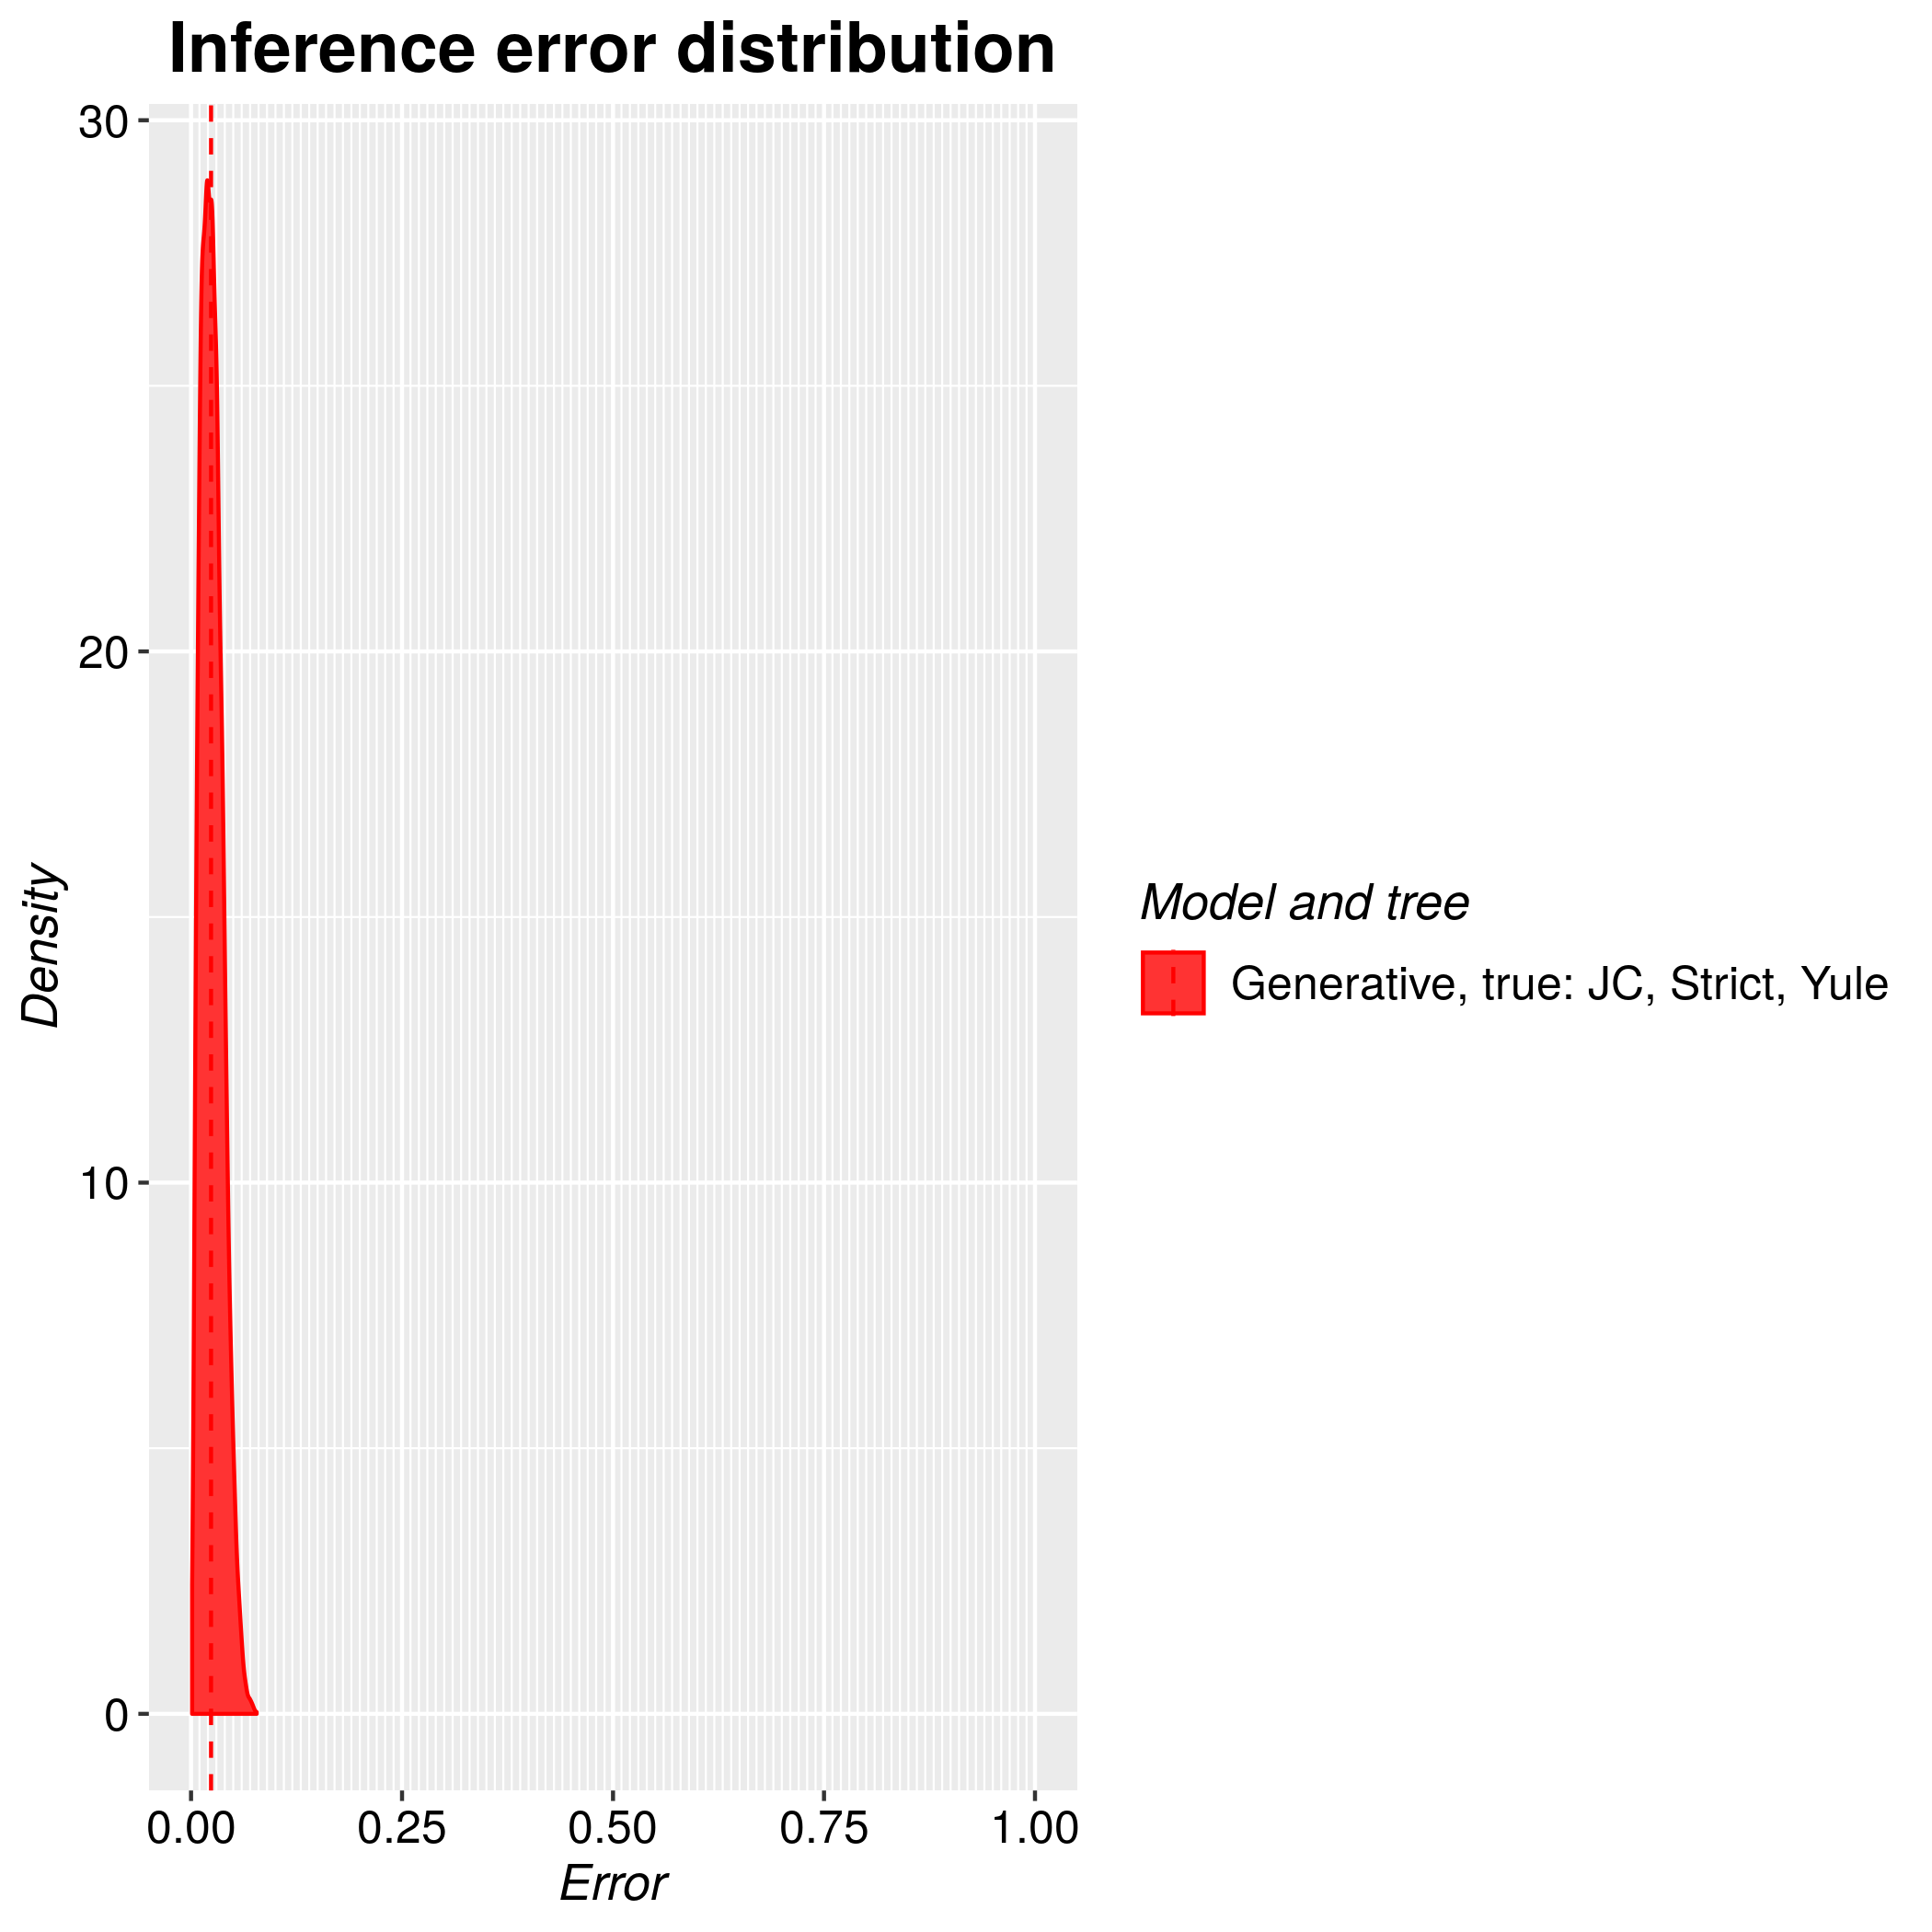
\includegraphics[width=\textwidth]{example_1/errors.png}
  \caption{
    The inference error made 
    when the generative and inference models are the same.
    The vertical dashed line indicates the median error.
  }
  \label{fig:example_1}
\end{figure}

The resulting error distribution, as shown Figure~\ref{fig:example_1},
shows the inference error 
when $\mathit{I}$ matches with the generative model given 
by $\mathit{A}$ and $\mathit{p_{G}^0}$.
This error distribution can serve as a control,
as it is obtained from a tree of which the tree prior is standard and known.
Obtaining this control is in fact an inherent part of \verb;pirouette;. 
We call it 'twinning' and we will demonstrate it at section
 \ref{Comparing to background noise}.

%%%%%%%%%%%%%%%%%%%%%%%%%%%%%%%%%%%%%%%%%%%%%%%%%%%%%%%%%%%%%%%%%%%%%%%%%%%%%%%%
\subsection{Comparing to other candidate models}
%%%%%%%%%%%%%%%%%%%%%%%%%%%%%%%%%%%%%%%%%%%%%%%%%%%%%%%%%%%%%%%%%%%%%%%%%%%%%%%%

In the previous example we selected the inference model $\mathit{I}$ to match 
with a known generative tree prior $\mathit{p_{G}^0}$.
However, a novel tree prior $\mathit{p_{G}}$, by our definition, is 
non-standard, and hence not part of a standard inference 
model (i.e. an inference model using a standard tree prior).
In such a case, the question is which standard tree prior should be used in 
the inference. In this example, not only we re-use our hand-picked 
inference model, but we also pick the best inference model from a set of 
inference models. With the 'best' inference model, we mean the model with 
the highest evidence (also known as marginal likelihood), based on the 
alignment. We show the procedure using \verb;pirouette; to answer a second 
research question: "What is the inference error made on a novel phylogeny when using the best inference model, in comparison to a hand-picked model?

\begin{table}
  \begin{tabular}{ | c | c | c | l | }
    \hline
    \textbf{model\_type} &
    \textbf{run\_if} &
    \textbf{do\_measure\_evidence} & 
    \textbf{inference model} \\ 
    \hline
    generative & always         & FALSE & JC, strict, Yule \\
    candidate  & best candidate & TRUE  & JC, strict, BD   \\
    candidate  & best candidate & TRUE  & JC, strict, CBS  \\
    ...        & ...            & ...   & ...              \\
    candidate  & best candidate & TRUE  & GTR, RLN, CCP    \\
    candidate  & best candidate & TRUE  & GTR, RLN, CEP    \\
    \hline
  \end{tabular}
  \caption{
    Inference conditions and model.
    JC: Jukes-Cantor site model.
    strict: strict clock model.
    Yule: Yule (pure-birth) tree prior.
    BD: birth-death tree prior.
    GTR: GTR site model.
    RLN: relaxed log-normal clock model.
    CBS: coalescent Bayesian Skyline tree prior.
    CCP: coalescent constant-population tree prior.
    CEP: coalescent exponential-population tree prior.
  }
  \label{tab:RQ2}
\end{table}

We will use the same tree as generated in \ref{lst:create_yule_tree}, as well 
as the same alignment parameters as shown 
in Listing~\ref{lst:create_alignment_params}.

Here we specify a different set of experiments: we
need to state that we already have an experiment for
the generative model, as well as that we want all the other inference models 
to compete. We call the competing models 'candidate models'.
As model selection is commonly performed on the full list of available 
candidate models, \verb;pirouette; has a dedicated function for this choice: \verb;create_all_experiments; creates a full set of 40 experiments, 
containing the inference models of all combinations of 4 site models, 
2 clock models and 5 tree priors. All we need to add is to exclude the 
inference model in the generative experiment:

\begin{lstlisting}[
  language = R, 
  floatplacement = ht, 
  frame = single, 
  label = {lst:create_all_experiments},
  caption = {
    Create all 40 candidate experiments, except for the inference model of the generative model.
  }
]
candidate_experiments <- create_all_experiments(
  exclude_model = generative_experiment$inference_model
)
\end{lstlisting}

We combine the generative and all the candidate models into one set of 
experiments:

\begin{lstlisting}[
  language = R, 
  floatplacement = ht, 
  frame = single, 
  label = {lst:create_all_experiments},
  caption = {
    Create a collection of experiments, with 1
    generative model, and 39 candidate models.
  }
]
experiments <- list(
  list(generative_experiment),
  candidate_experiments
)
\end{lstlisting}

We can now create the complete \verb;pirouette; parameter set in the usual 
way (which is the same as Listing~\ref{lst:create_pir_params}, but using the 
defaults):

\begin{lstlisting}[
  language = R,
  floatplacement = ht,
  frame = single,
  label = {lst:create_pir_params_defaults},
  caption = Create a \texttt{pir\_params} with many defaults.
]
pir_params <- create_pir_params(
  alignment_params = alignment_params,
  experiments = experiments
)
\end{lstlisting}

We run \verb;pirouette; (Listing~\ref{lst:pir_run}) 
and plot the results (Listing~\ref{lst:pir_plot}) in Figure~\ref{fig:example_2}.

\begin{figure}[H]
  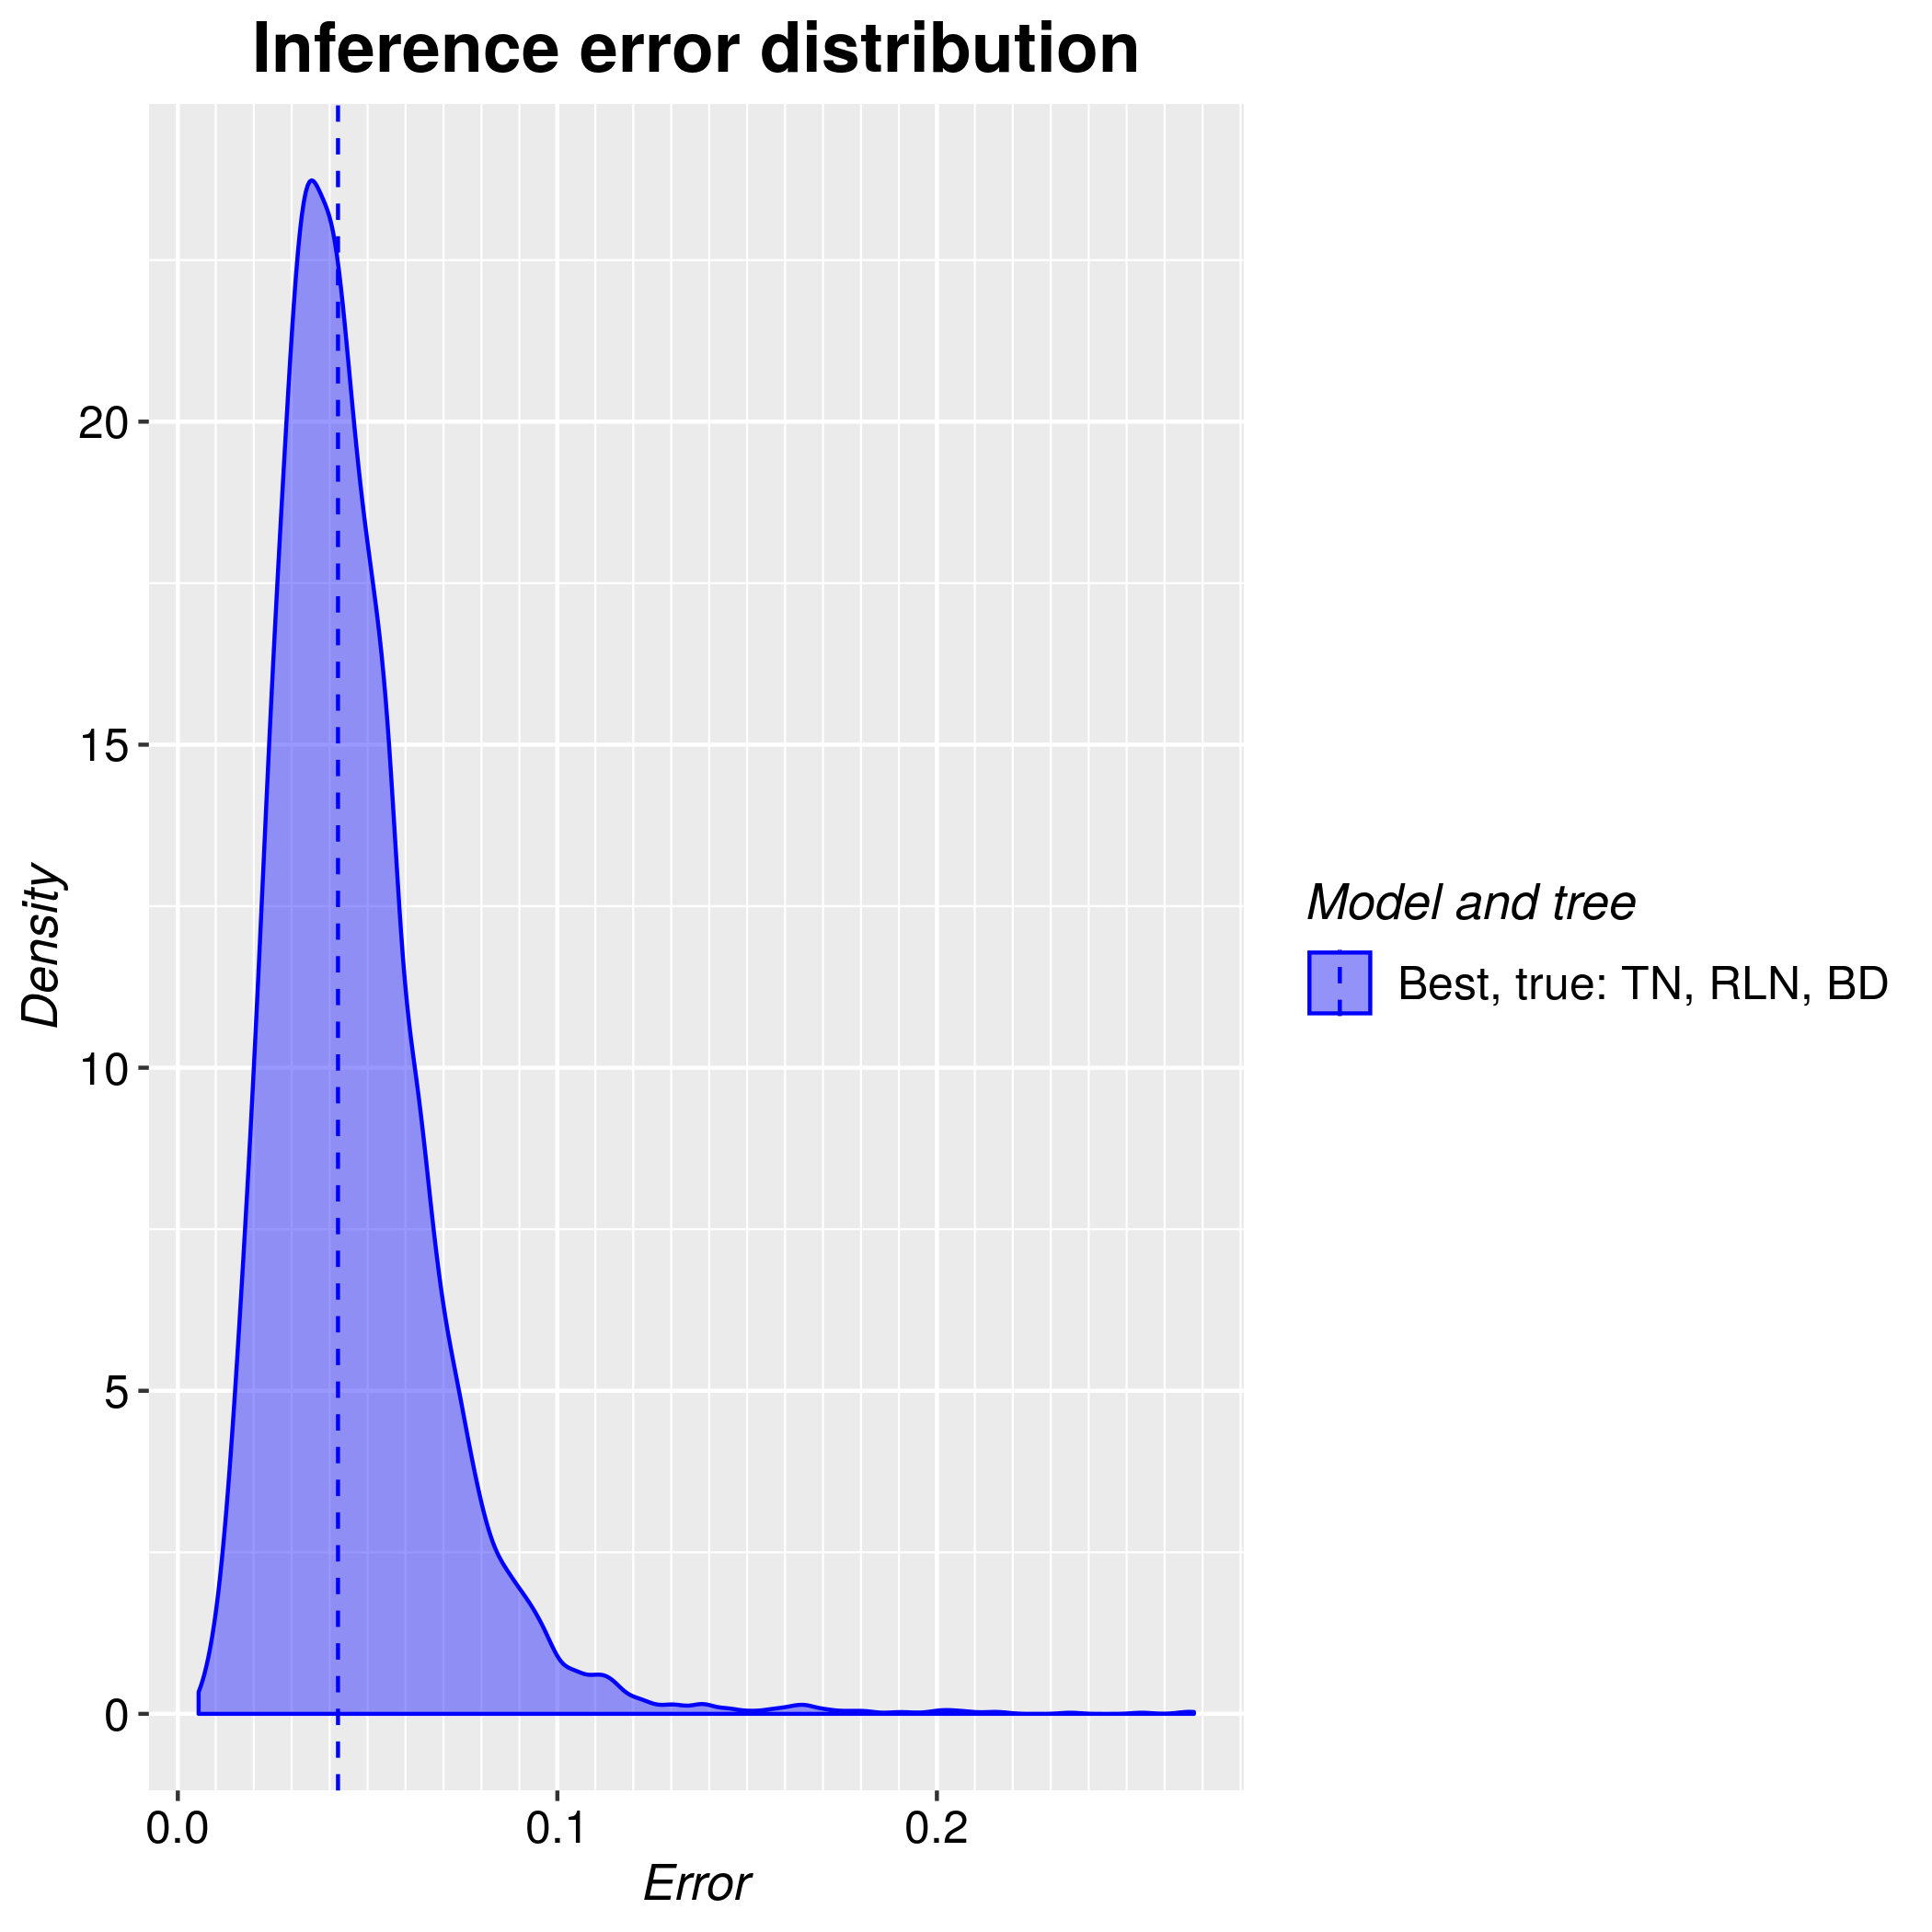
\includegraphics[width=\textwidth]{example_2/errors.png}
  \caption{
    The inference error for both generative and best candidate inference models.
    Vertical dashed lines show the median error value per distribution.
  }
  \label{fig:example_2}
\end{figure}

%%%%%%%%%%%%%%%%%%%%%%%%%%%%%%%%%%%%%%%%%%%%%%%%%%%%%%%%%%%%%%%%%%%%%%%%%%%%%%%%
\subsection{Comparing to background noise}\label{Comparing to background noise}
%%%%%%%%%%%%%%%%%%%%%%%%%%%%%%%%%%%%%%%%%%%%%%%%%%%%%%%%%%%%%%%%%%%%%%%%%%%%%%%%

So far we have measured the inference error on a tree
generated according to a known (and standard) tree prior. 
The goal of \verb;pirouette; is to measure the impact of a novel tree prior.
To do so, in this example, we will use a tree generated by a non-standard 
tree prior, assumed to be closely related to the Yule tree prior.
To measure the impact of the tree prior, we measure both the baseline 
error (that serves as a control) and the full inference error: it is their 
difference that shows the impact of the tree prior.
To do so, we use a twin tree (see Subsection~\ref{subsec:twinning}) for 
each of the generative and best candidate model.
The research question this example answers is:
"What is the inference error made from a phylogeny, 
for both a generative model and a best candidate model, compared to the 
background noise?"

We start from the tree generated by a non-standard (and unknown) tree prior, having six taxa and a crown age of ten:
\begin{lstlisting}[
  language = R, 
  floatplacement = ht,
  frame = single, 
  label = {lst:unknown_phylogeny},
  caption = A phylogeny generated by an unknown diversification model.
]
phylogeny  <- ape::read.tree(
  text = "(((A:8, B:8):1, C:9):1, ((D:8, E:8):1, F:9):1);"
)
\end{lstlisting}
\begin{figure}[H]
  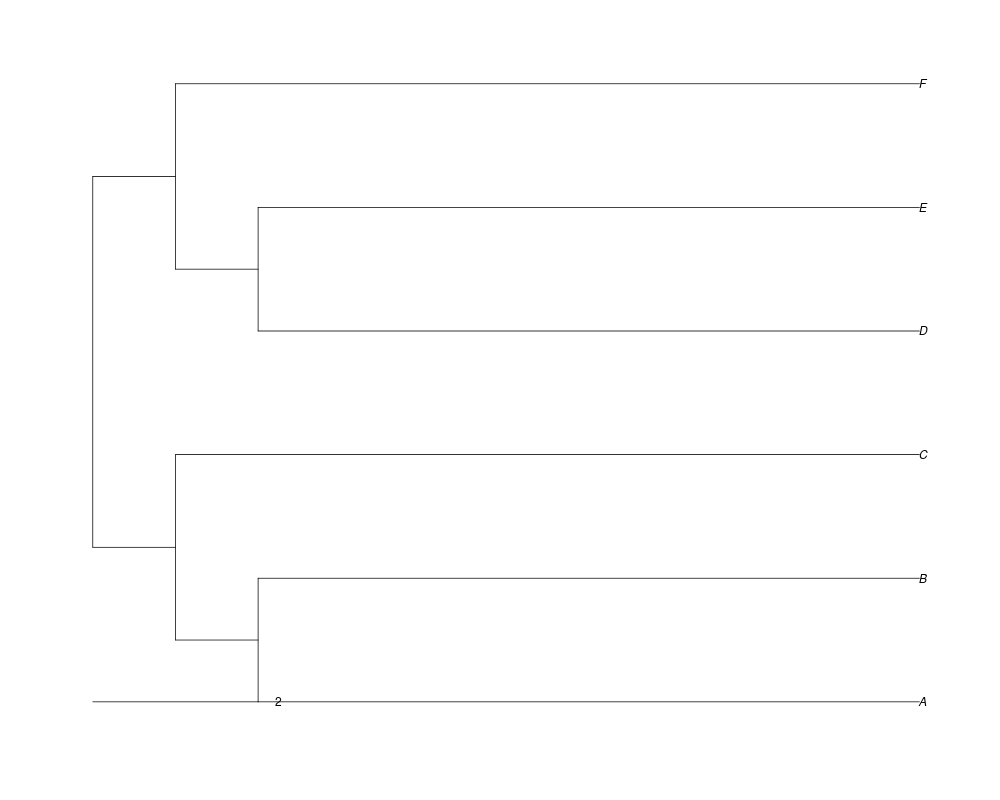
\includegraphics[width=\textwidth]{example_6/true_tree.png}
  \caption{The tree derived from an unknown diversification process, 
    as created by listing~\ref{lst:unknown_phylogeny}.
  }
\end{figure}

Most of the other settings are the same as before: we re-use the alignment parameters (Listing~\ref{lst:create_alignment_params}), as well as the experiments (Listing~\ref{lst:create_all_experiments}).
This time, however, we enable twinning (see Subsection~\ref{subsec:twinning}),
by creating twinning parameters.
Creating these parameters is trivial with the default settings.
For clarity, however, we explicitly show the most important arguments:

\begin{lstlisting}[
  language = R,
  floatplacement = ht,
  frame = single,
  label = {lst:create_twinning_params},
  caption = Create the default twinning parameters.
]
twinning_params <- create_twinning_params(
  twin_model = "bd", 
  method = "random_tree"
)
\end{lstlisting}

We combine all the parameters using \verb;create_pir_params;:

\begin{lstlisting}[
  language = R,
  floatplacement = ht,
  frame = single,
  label = {lst:create_pir_params_with_twinning},
  caption = Create the default twinning parameters.
]
pir_params <- create_pir_params(
  alignment_params = alignment_params,
  experiments = experiments,
  twinning_params = twinning_params
)
\end{lstlisting}

We run \verb;pirouette; (Listing~\ref{lst:pir_run}) 
and plot the results (Listing~\ref{lst:pir_plot}).
The output is shown in Figure~\ref{fig:example_3}.

\begin{figure}[H]
  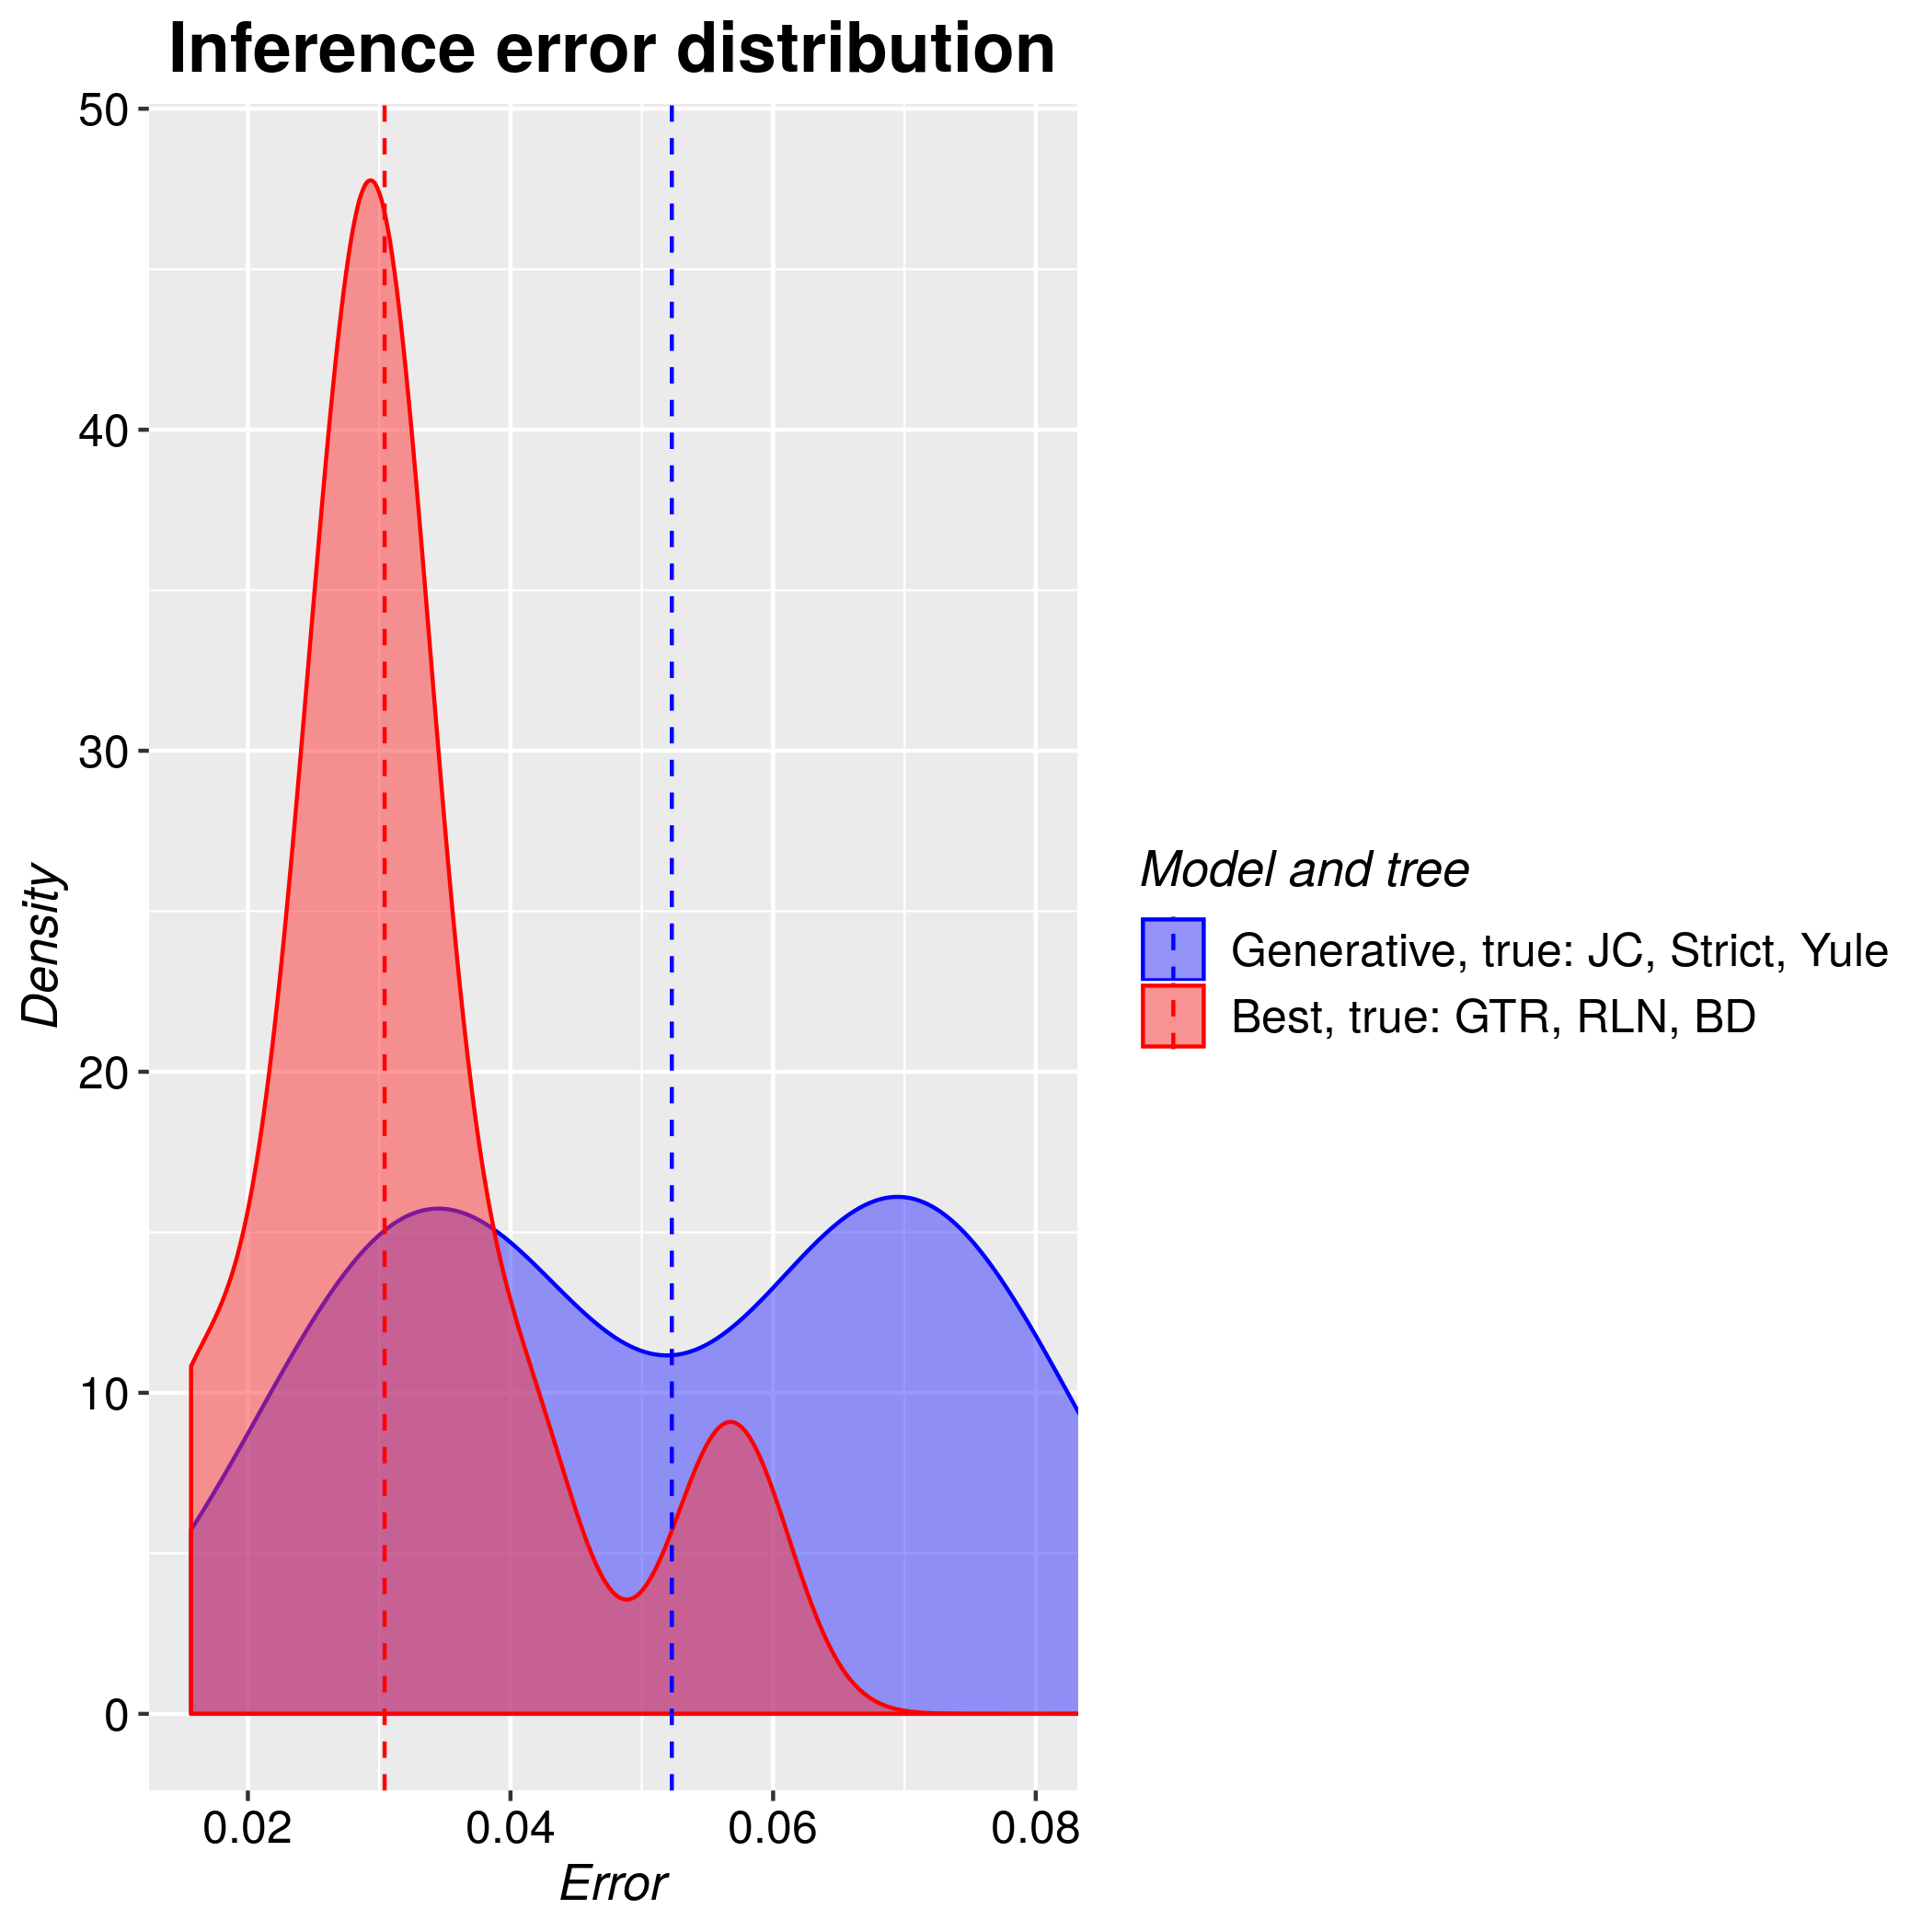
\includegraphics[width=\textwidth]{example_6/errors.png}
  \caption{
    The inference error made 
    for both a generative tree prior and best candidate model
    compared with the error obtained for the twin tree.
    Here, the 'twin' tree shows the baseline inference error.
    Vertical dashed lines show the median error value per distribution.
  }
  \label{fig:example_3}
\end{figure}

%%%%%%%%%%%%%%%%%%%%%%%%%%%%%%%%%%%%%%%%%%%%%%%%%%%%%%%%%%%%%%%%%%%%%%%%%%%%%%%%
\section{Discussion}
%%%%%%%%%%%%%%%%%%%%%%%%%%%%%%%%%%%%%%%%%%%%%%%%%%%%%%%%%%%%%%%%%%%%%%%%%%%%%%%%

We showed how to use \verb;pirouette; to quantify the importance of a 
tree prior in Bayesian phylogenetics, using the simplest generative tree 
prior possible.
In principle any other (more complex) generative tree prior can be tested, 
but we chose to provide the simplest (and fastest to run) examples.
All examples used only one original tree,
where any speciation process produces a whole range of trees.
One tree is not enough to determine the impact of a tree prior 
on Bayesian inference.
However, if the same procedure were repeated and performed on a 
distribution with a sufficient number of generative trees, 
it would constitute a quantitative and effective assessment of the 
quality of the inference.
Also a twin tree does not always result in a lower error distribution,
due to the stochasticity in generating the twin tree.

In conclusion, \verb;pirouette; can directly show the comparison 
between the results obtained 
adopting a new generative prior as compared to the Bayesian inference error
when operating on a tree generated under a known and standard tree 
prior (the twin tree).
From such results an user can estimate whether or not a new tree prior, 
tailored on the generative process, is needed. 
If this were indeed the case, one could rightly implement 
their novel tree prior as an addition to 
their favorite Bayesian inference tool.

\begin{table}
  \begin{tabular}{ | r | c | c | c | }
    \hline
    \textbf{Compare with} & \textbf{TB} & \textbf{WG} & \textbf{WB} \\ 
    \hline
    \textbf{TG} & Y & Y & N \\
    \textbf{TB} & . & N & Y \\
    \textbf{WG} & . & . & Y \\
    \textbf{WB} & . & . & . \\
    \hline
  \end{tabular}
  \caption{
    Error distributions that are relevant to compare.
    TG: true tree, generative model.
    TB: true tree, best candidate model.
    WG: twin tree, generative model.
    WB: twin tree, best candidate model.
  }
  \label{tab:relevant_comparisions}
\end{table}

\begin{table}
  \begin{tabular}{ | r | c | p{9cm} | }
    \hline
    \textbf{Condition} & \textbf{Expectation} & \textbf{Interpretation} \\ 
    \hline
    %%%%%%%%%%%%%%%%%%%%%%%%%%%%%%%%%%%%%%%%%%%%%%%%%%%%%%%%%%%%%%%%%%%%%%%%%%%%
    \textbf{$TG > TB$}       & Unexpected & Novel tree prior is more related to 
      best candidate than hand-picked tree prior \\
    %%%%%%%%%%%%%%%%%%%%%%%%%%%%%%%%%%%%%%%%%%%%%%%%%%%%%%%%%%%%%%%%%%%%%%%%%%%%
    \textbf{$TG \approx TB$} & Possible   & Hand-picked tree prior is just as 
      suitable as the best candidate tree prior \\
    %%%%%%%%%%%%%%%%%%%%%%%%%%%%%%%%%%%%%%%%%%%%%%%%%%%%%%%%%%%%%%%%%%%%%%%%%%%%
    \textbf{$TG < TB$}       & Expected   & Hand-picked tree prior is the most 
      related tree prior \\
    %%%%%%%%%%%%%%%%%%%%%%%%%%%%%%%%%%%%%%%%%%%%%%%%%%%%%%%%%%%%%%%%%%%%%%%%%%%%
    \hline
    %%%%%%%%%%%%%%%%%%%%%%%%%%%%%%%%%%%%%%%%%%%%%%%%%%%%%%%%%%%%%%%%%%%%%%%%%%%%
    \textbf{$TG > WG$}       & Unknown    & Novel tree prior important \\
    %%%%%%%%%%%%%%%%%%%%%%%%%%%%%%%%%%%%%%%%%%%%%%%%%%%%%%%%%%%%%%%%%%%%%%%%%%%%
    \textbf{$TG \approx WG$} & Unknown    & Novel tree prior unimportant \\
    %%%%%%%%%%%%%%%%%%%%%%%%%%%%%%%%%%%%%%%%%%%%%%%%%%%%%%%%%%%%%%%%%%%%%%%%%%%%
    \textbf{$TG < WG$}       & Unexpected & Twinning procedure increases 
      inference errors when using hand-picked tree prior \\
    %%%%%%%%%%%%%%%%%%%%%%%%%%%%%%%%%%%%%%%%%%%%%%%%%%%%%%%%%%%%%%%%%%%%%%%%%%%%
    \hline
    %%%%%%%%%%%%%%%%%%%%%%%%%%%%%%%%%%%%%%%%%%%%%%%%%%%%%%%%%%%%%%%%%%%%%%%%%%%%
    \textbf{$TB > WB$}       & Expected   & Impact of novel tree prior cannot 
      be compensated for by model selection: twin tree with low likelihood? \\
    %%%%%%%%%%%%%%%%%%%%%%%%%%%%%%%%%%%%%%%%%%%%%%%%%%%%%%%%%%%%%%%%%%%%%%%%%%%%
    \textbf{$TB \approx WB$} & Possible   & Best candidate tree priors perform 
      equally well in true and twin tree: true and twin tree similar? \\
    %%%%%%%%%%%%%%%%%%%%%%%%%%%%%%%%%%%%%%%%%%%%%%%%%%%%%%%%%%%%%%%%%%%%%%%%%%%%
    \textbf{$TB < WB$}       & Unexpected & Twinning procedure increases 
      inference errors  when using best tree prior candidate \\
    %%%%%%%%%%%%%%%%%%%%%%%%%%%%%%%%%%%%%%%%%%%%%%%%%%%%%%%%%%%%%%%%%%%%%%%%%%%%
    \hline
    %%%%%%%%%%%%%%%%%%%%%%%%%%%%%%%%%%%%%%%%%%%%%%%%%%%%%%%%%%%%%%%%%%%%%%%%%%%%
    \textbf{$WG > WB$}       & Unexpected & Hand-picked tree prior (that equals 
      the twinning tree prior!) worse than best candidate tree prior \\
    %%%%%%%%%%%%%%%%%%%%%%%%%%%%%%%%%%%%%%%%%%%%%%%%%%%%%%%%%%%%%%%%%%%%%%%%%%%%
    \textbf{$WG \approx WB$} & Possible   & Twin tree fits equally well to the 
      hand-picked and best candidate tree prior  \\
    %%%%%%%%%%%%%%%%%%%%%%%%%%%%%%%%%%%%%%%%%%%%%%%%%%%%%%%%%%%%%%%%%%%%%%%%%%%%
    \textbf{$WG < WB$}       & Expected   & Hand-pick tree prior (that equals 
      the twinning tree prior) performs as expected \\
    %%%%%%%%%%%%%%%%%%%%%%%%%%%%%%%%%%%%%%%%%%%%%%%%%%%%%%%%%%%%%%%%%%%%%%%%%%%%
    \hline
  \end{tabular}
  \caption{
    Interpretation of the different error distributions.
    This assumes that the operators ($<$, $\approx$ and $>$) to compare
    distributions are defined.
    TG: true tree, generative model.
    TB: true tree, best candidate model.
    WG: true tree, generative model.
    WB: true tree, best candidate model.
  }
  \label{tab:interpretation}
\end{table}

%%%%%%%%%%%%%%%%%%%%%%%%%%%%%%%%%%%%%%%%%%%%%%%%%%%%%%%%%%%%%%%%%%%%%%%%%%%%%%%%
\section{pirouette resources}
%%%%%%%%%%%%%%%%%%%%%%%%%%%%%%%%%%%%%%%%%%%%%%%%%%%%%%%%%%%%%%%%%%%%%%%%%%%%%%%%

\verb;pirouette; is free, libre and open source software available at 
\url{http://github.com/richelbilderbeek/pirouette},
licensed under the GNU General Public License version 3.
\verb;pirouette; depends on multiple packages, which are:
\verb;babette; (\cite{bilderbeek2018babette}),
\verb;becosys; (\cite{becosys}),
\verb;DDD; (\cite{DDD}),
\verb;devtools; (\cite{devtools}),
\verb;geiger; (\cite{geiger}),
\verb;ggplot2; (\cite{ggplot2}),
\verb;knitr; (\cite{knitr}),
\verb;lintr; (\cite{lintr}),
\verb;mcbette; (\cite{mcbette}),
\verb;nLTT; (\cite{nLTT}),
\verb;PBD; (\cite{PBD}),
\verb;phangorn; (\cite{phangorn}),
\verb;phytools; (\cite{phytools}),
\verb;rappdirs; (\cite{rappdirs}),
\verb;rmarkdown; (\cite{rmarkdown}),
\verb;Rmpfr; (\cite{Rmpfr}),
\verb;stringr; (\cite{stringr}),
\verb;subplex; (\cite{subplex}),
\verb;TESS; (\cite{TESS}),
\verb;testit; (\cite{testit}), 
\verb;testthat; (\cite{testthat}) and
\verb;tidyr; (\cite{tidyr}).

\verb;pirouette;'s development takes place on GitHub,
\url{https://github.com/richelbilderbeek/pirouette},
which allows submitting bug reports, requesting features, 
or adding code. To ensure a high quality, \verb;pirouette; 
uses a continuous integration service, has a code coverage of 100\%
and enforces the most commonly used R style guide (\cite{style_guide}).

\verb;pirouette;'s is extensively documented on its website,
its documentation and its vignettes.
The \verb;pirouette; website is a good starting point to learn
how to use \verb;pirouette;, as it links to tutorials and videos.
The \verb;pirouette; package documentation describes
all functions and liberally links to related functions.
All exported functions show a minimal example as part of their documentation.
The \verb;pirouette; vignette demonstrates extensively how 
to use \verb;pirouette; in a more lightly written way. 

%%%%%%%%%%%%%%%%%%%%%%%%%%%%%%%%%%%%%%%%%%%%%%%%%%%%%%%%%%%%%%%%%%%%%%%%%%%%%%%%
\section{Citation of pirouette}
%%%%%%%%%%%%%%%%%%%%%%%%%%%%%%%%%%%%%%%%%%%%%%%%%%%%%%%%%%%%%%%%%%%%%%%%%%%%%%%%

To cite \verb;pirouette; this article from within R, use:

\begin{lstlisting}[language=R]
> citation("pirouette")
\end{lstlisting}

%%%%%%%%%%%%%%%%%%%%%%%%%%%%%%%%%%%%%%%%%%%%%%%%%%%%%%%%%%%%%%%%%%%%%%%%%%%%%%%%
\section{Acknowledgments}
%%%%%%%%%%%%%%%%%%%%%%%%%%%%%%%%%%%%%%%%%%%%%%%%%%%%%%%%%%%%%%%%%%%%%%%%%%%%%%%%

We would like to thank the Center for Information Technology of the University 
of Groningen for its support and for providing access to the Peregrine 
high performance computing cluster. 
We thank the Netherlands 
Organization for Scientific Research (NWO) for financial support 
through a VICI grant awarded to RSE.

%%%%%%%%%%%%%%%%%%%%%%%%%%%%%%%%%%%%%%%%%%%%%%%%%%%%%%%%%%%%%%%%%%%%%%%%%%%%%%%%
\section{Data Accessibility}
%%%%%%%%%%%%%%%%%%%%%%%%%%%%%%%%%%%%%%%%%%%%%%%%%%%%%%%%%%%%%%%%%%%%%%%%%%%%%%%%

All code is archived at 
\url{http://github.com/richelbilderbeek/pirouette_article},
with DOI \url{https://doi.org/12.3456/zenodo.1234567}.

%%%%%%%%%%%%%%%%%%%%%%%%%%%%%%%%%%%%%%%%%%%%%%%%%%%%%%%%%%%%%%%%%%%%%%%%%%%%%%%%
\section{Authors' contributions}
%%%%%%%%%%%%%%%%%%%%%%%%%%%%%%%%%%%%%%%%%%%%%%%%%%%%%%%%%%%%%%%%%%%%%%%%%%%%%%%%

RJCB, GL and RSE conceived the idea for the package. 
RJCB created and tested the package, and wrote the first draft of the manuscript.
GL tested the package and contributed to revisions.
RSE contributed to revisions.

%%%%%%%%%%%%%%%%%%%%%%%%%%%%%%%%%%%%%%%%%%%%%%%%%%%%%%%%%%%%%%%%%%%%%%%%%%%%%%%%
% Bibliography
%%%%%%%%%%%%%%%%%%%%%%%%%%%%%%%%%%%%%%%%%%%%%%%%%%%%%%%%%%%%%%%%%%%%%%%%%%%%%%%%
% MEE style
\bibliographystyle{mee}
\bibliography{article}
%%%%%%%%%%%%%%%%%%%%%%%%%%%%%%%%%%%%%%%%%%%%%%%%%%%%%%%%%%%%%%%%%%%%%%%%%%%%%%%%
